%%%% IJCAI--ECAI 26 Paper
\typeout{IJCAI--ECAI 26 Paper}

\documentclass{article}
\pdfpagewidth=8.5in
\pdfpageheight=11in

% The file ijcai26.sty is the IJCAI style file
\usepackage{ijcai26}

% Use the postscript times font!
\usepackage{times}
\usepackage{soul}
\usepackage{url}
\usepackage[hidelinks]{hyperref}
\usepackage[utf8]{inputenc}
\usepackage[T1]{fontenc}  % Fix for special characters like ą in author names
\usepackage[small]{caption}
\usepackage{amsmath}
\usepackage{amssymb}
% \usepackage{titling}

\usepackage{placeins}
\usepackage{amsthm}
\usepackage{booktabs}
% Use algorithm2e only (not algorithm + algorithmic which conflicts)
\usepackage[ruled,vlined,linesnumbered]{algorithm2e}  % For \KwIn, \KwOut, \ForEach, etc.
\usepackage[switch]{lineno}
\usepackage{subcaption}
\usepackage{tabularx}
\usepackage{xcolor}
\usepackage{tcolorbox}
\usepackage{float}
\usepackage{placeins}       % thêm để dùng \FloatBarrier (khuyên dùng)

% Comment out this line in the camera-ready submission
\linenumbers

\urlstyle{same}

% Define theorem environments
\newtheorem{example}{Example}
\newtheorem{theorem}{Theorem}

% Custom commands from original paper
\newcommand{\ty}{\textcolor{yellow}}
\newcommand{\tr}{\textcolor{red}}
\newcommand{\tb}{\textcolor{blue}}

% PDF Info
\pdfinfo{
/TemplateVersion (IJCAI.2026.0)
}

%\title{Understanding LLM Agent behaviors via Game Theory: Strategy Recognition, Biases and Multi-Agent Dynamics}

\title{More at Stake: How Payoff and Language Shape LLM Agent Strategies in Cooperation Dilemmas}



% Multiple author syntax for IJCAI
\author{
Trung-Kiet Huynh$^{1,3,\dagger}$\and
Dao-Sy Duy-Minh$^{1,3,\dagger}$\and
Thanh-Bang Cao$^{2,3}$\and
Phong-Hao Le$^{2,3}$\and
Hong-Dan Nguyen$^{2,3}$\And
Nguyen Lam Phu Quy$^{1,3}$\and
Minh-Luan Nguyen-Vo$^{2,3}$\and
Hong-Phat Pham$^{2,3}$\and
Pham Phu Hoa$^{1,3}$\and
Thien-Kim Than$^{2,3}$\And
Chi-Nguyen Tran$^{2,3}$\and
Huy Tran$^{2,3}$\and
Gia-Thoai Tran-Le$^{2,3}$\and
Alessio Buscemi$^{4}$\and
Le Hong Trang$^{2,3,\star}$\and
The Anh Han$^{5,\star}$\\
\affiliations
$^1$Faculty of Information Technology, University of Science (HCMUS), Vietnam\\
$^2$Faculty of Computer Science and Engineering, Ho Chi Minh City University of Technology (HCMUT), Vietnam\\
$^3$Vietnam National University - Ho Chi Minh City (VNU-HCM), Vietnam\\
$^4$Luxembourg Institute of Science and Technology, Luxembourg\\
$^5$School of Computing, Engineering and Digital Technologies, Teesside University, UK\\
$^\dagger$Equal Contribution, $^\star$Corresponding authors\\
\emails
23122039@student.hcmus.edu.vn,
23122041@student.hcmus.edu.vn,
bang.caothanh455@hcmut.edu.vn,
hao.lephong@hcmut.edu.vn,
nhdan.sdh232@hcmut.edu.vn,
23122048@student.hcmus.edu.vn,
luan.nguyenvm@hcmut.edu.vn,
phat.phamhong@hcmut.edu.vn,
23122030@student.hcmus.edu.vn,
kim.thanthien04@hcmut.edu.vn,
23122044@student.hcmus.edu.vn,
tranhuy@hcmut.edu.vn,
thoai.trantlgt2610@hcmut.edu.vn,
t.han@tees.ac.uk,
lhtrang@hcmut.edu.vn
}

\date{}

\begin{document}

\maketitle
% \setlength{\droptitle}{-5cm}
\begin{abstract}
As LLMs increasingly act as autonomous agents in interactive and multi-agent settings, understanding their strategic behavior is critical for safety, coordination, and AI-driven social and economic systems. 
We investigate how payoff magnitude and linguistic context shape LLM strategies in repeated social dilemmas, using a payoff-scaled Prisoner's Dilemma to isolate sensitivity to incentive strength.
Across models and languages, we observe consistent behavioral patterns, including incentive-sensitive conditional strategies and cross-linguistic divergence. To interpret these dynamics, we train supervised classifiers on canonical repeated-game strategies and apply them to LLM decisions, revealing systematic, model- and language-dependent behavioral intentions, with linguistic framing sometimes matching or exceeding architectural effects. Our results provide a unified framework for auditing LLMs as strategic agents and highlight cooperation biases with direct implications for AI governance and multi-agent system design.
\end{abstract}

\section{Introduction}
\label{sec:intro}

Large language models (LLMs) are increasingly deployed as \emph{agents} in recommendation systems, negotiation tools, and multi-agent assistants~\cite{tessler2024ai,hammond2025multi}. In these settings, LLMs face \emph{cooperation dilemmas} in which behavior emerges from strategic interactions rather than isolated model outputs. Empirical studies show that such behavior is shaped by training, prompting, role assignment, and linguistic framing, with direct implications for safety, coordination, and AI governance~\cite{lu2024llms,akata2025,fontana2025nicer}.
Equally critical is the adaptability of their cooperative strategies to varying costs and benefits (payoff stakes), as this directly influences AI system outcomes across a spectrum of real-world scenarios \cite{hammond2025multi}.

A growing body of work evaluates LLMs through game-theoretic lenses, particularly via matrix and repeated games, revealing systematic departures from Nash equilibria, persistent cooperative biases, and sensitivity to contextual factors such as language and incentives~\cite{akata2025,sun2025gtllm_survey,mao2025alympics,pal2026strategiescooperationdefectionlarge,willis2025will,fan2024can,pires2025large}. FAIRGAME~\cite{buscemi2025fairgame} provides a controlled experimental framework for probing these effects across models, languages, and personalities. However, most existing evaluations focus on aggregate outcomes, such as cooperation rates or payoff distributions, and do not directly model the \emph{behavioral intentions} underlying observed actions.

Evaluating strategic behavior at the level required for governance and alignment therefore demands methods that go beyond surface-level outputs. Drawing on behavioral and evolutionary game theory, we conceptualize behavioral intention as an agent’s \emph{strategy}: a decision rule mapping interaction histories to subsequent actions~\cite{han2011role,diStefanoIntention2023,Han2012ALIFEjournal,fujimoto2019functional}. Classical canonical strategies in repeated games, such as Always Cooperate (ALLC), Always Defect (ALLD), Tit-for-Tat (TFT), and Win-Stay–Lose-Shift (WSLS)~\cite{Axelrod1980Effective,sigmund:2010bo}, provide an interpretable vocabulary for such intentions. Prior work has shown that these strategies can be inferred from noisy behavioral trajectories using supervised learning~\cite{han2011role,diStefanoIntention2023}, and extended using probabilistic models to capture mixed or stochastic behavior~\cite{inferenceStrategies}.

In parallel, recent studies highlight that LLM behavior is not invariant across languages \cite{buscemi2025fairgame}. Strategic reasoning, risk sensitivity, and cooperation patterns have been shown to depend on linguistic framing, sometimes with effects comparable in magnitude to architectural differences~\cite{loreheydari2024strategic,buscemi2025llms}. This raises the question of whether behavioral intentions (or strategies used by LLM agents) inferred from gameplay are themselves language-dependent, and whether such dependencies introduce systematic biases in multi-agent settings.

This work builds on and extends these strands of research. Our experimental design incorporates a payoff-scaled Prisoner’s Dilemma that systematically  varies the \emph{stakes} (i.e. magnitude) of cooperation while preserving the underlying strategic structure. Moreover, using synthetic repeated-game trajectories \cite{han2011role}, we train supervised intention classifiers and apply them to LLM-generated gameplay logs to infer canonical strategies. This allows us to address two important questions:  
1) Do LLM agents systematically change cooperative behavior as payoff stakes vary, and how does this differ across models and languages?  
2) Can LLM behavioral intentions be reliably classified using supervised learning, and what systematic biases emerge across models and languages?


Our approach complements and extends recent long-horizon studies of repeated games with LLMs. In particular, Fontana et al.~\cite{fontana2025nicer} analyse 100-round interactions and introduce the Strategy Frequency Estimation Method (SFEM) to recover rich strategic archetypes, including Grim Trigger, Generous Tit-for-Tat, and extortionate strategies, achieving high population-level accuracy. %By contrast, our 10-round horizon enables rapid exploration of payoff scaling and multilingual effects, trading the ability to detect complex conditional strategies for interpretable, pointwise estimates of canonical intentions.
Our approach employs a 10-round horizon, which is  designed to enable direct exploration of payoff-scaling and multilingual effects - the core contextual factors of our study. This design, while trading off the capacity to discern complex, multi-stage conditional strategies, allows us to obtain highly interpretable, pointwise estimates of canonical intentions.%, offering focused insights into LLM behavioral responses to immediate changes.

Finally, while human behavioral baselines in repeated Prisoner’s Dilemma are well studied~\cite{inferenceStrategies,akata2025,Axelrod1980Effective,krockow2016cooperation}, systematic comparisons under matched experimental conditions remain largely absent from LLM evaluations. Human cooperation rates and strategy distributions vary with incentives, culture, and framing. Our findings of incentive and payoff-stakes sensitive cooperation and cross-linguistic divergence echo these patterns, but without direct human baselines, we do not claim behavioral equivalence. Instead, we position intention classification as a diagnostic tool for identifying systematic structure and bias in LLM strategic behavior, providing a foundation for future comparative and governance-oriented analyses.


% \section{Introduction}
% \label{sec:intro}

% Large language models (LLMs) are increasingly deployed as \emph{agents} in recommendation systems, negotiation tools, and multi-agent assistants~\cite{tessler2024ai,hammond2025multi}. In these settings, LLMs face \emph{cooperation dilemmas} where their  behavior and strategies-shaped by training, prompting, and role assignment-have profound implications for safety, coordination, and AI governance~\cite{lu2024llms,akata2025,fontana2025nicer}.

% Evaluating such strategic behavior requires methods that capture not only what LLMs output, but the underlying \emph{intentions} guiding their decisions. 
% Drawing from repeated-game theory, we conceptualise `behavioral intention' as an agent's strategy: a decision rule that maps interaction histories to subsequent actions~\cite{diStefanoIntention2023,Han2012ALIFEjournal,han2011role}. 
%  Classical canonical strategies in repeated games such as Always Cooperate (AllC), Always Defect (AllD), Tit-for-Tat (TFT), and Win-Stay-Lose-Shift (WSLS) ~\cite{Axelrod1980Effective,sigmund:2010bo} can then be  recognised  from noisy interaction histories. This is achieved by employing a corpus-based intention recognition model, which uses supervised machine learning to effectively treat behavioral intention as a learnable and classifiable object.
% %Classical strategies Always Cooperate (ALLC), Always Defect (ALLD), Tit-for-Tat (TFT), Win-Stay-Lose-Shift (WSLS)~\cite{Axelrod1980Effective,sigmund:2010bo}-can be recognised from noisy trajectories via machine learning, enabling behavioral intention to be treated as a learnable object.

% We extend FAIRGAME~\cite{buscemi2025fairgame} with a payoff-scaled Prisoner’s Dilemma that varies the stakes of cooperation while preserving strategic structure, and apply supervised classifiers trained on synthetic trajectories to LLM gameplay logs to address two research questions: RQ1) Do LLM agents systematically change cooperative behavior as payoff stakes vary, and how does this differ across models and languages?; RQ2)  Can we classify LLM behavioral intentions using ML, and what systematic biases emerge across models, languages, and roles?

% % In this work, we extend FAIRGAME~\cite{buscemi2025fairgame} with a payoff-scaling module for the Prisoner's Dilemma, manipulating the \emph{stakes} of cooperation while preserving strategic structure. We then train classifiers on synthetic trajectories and apply them to LLM gameplay logs to infer canonical strategies. This addresses:
% % \begin{itemize}
% %   \item \textbf{RQ1.} Do LLM agents systematically change cooperative behavior as payoff stakes vary, and how does this differ across models and languages?
% %   \item \textbf{RQ2.} Can we classify LLM behavioral intentions using ML, and what systematic biases emerge across models, languages, and roles?
% % \end{itemize}

% % The following sections develop these contributions: Section~\ref{sec:related} reviews related work; Section~\ref{sec:methodology} describes our extensions; Section~\ref{sec:results} reports empirical results; and the final sections discuss limitations and future directions.

% \section{Related Work}
% \label{sec:related}

% \textbf{Game-Theoretic Evaluation of LLMs.} Recent work probes LLMs as strategic agents in matrix games, revealing systematic departures from Nash equilibria and stable cooperative biases~\cite{akata2025,fontana2025nicer,sun2025gtllm_survey,mao2025alympics}. FAIRGAME~\cite{buscemi2025fairgame} provides a controlled framework for measuring biases and cooperation across models, languages, and personalities, but does not include methods for behavioral intention analysis.

% \textbf{Strategy Inference in Repeated Games.} Di Stefano et al.~\cite{diStefanoIntention2023} demonstrate that canonical IPD strategies can be inferred from noisy trajectories using supervised learning. Montero-Porras et al.~\cite{inferenceStrategies} extend this with HMMs for capturing mixed behaviors. We build on this tradition by applying intent recognition to LLM-generated trajectories.

% \textbf{Cross-Lingual Biases in LLMs.} LLMs exhibit language-dependent biases in reasoning and decision-making~\cite{loreheydari2024strategic,buscemi2025llms}. Our work systematically evaluates whether linguistic framing affects strategic behavior in repeated games, finding effects that sometimes rival architectural differences.

% \textbf{Long-Horizon Repeated Games.} Fontana et al.~\cite{fontana2024nicer,fontana2025nicer} conduct 100-round iterated Prisoner's Dilemma experiments, revealing richer strategic archetypes including Grim Trigger (GRIM), Generous Tit-for-Tat (GTFT), and extortionate Zero-Determinant strategies. Their Strategy Frequency Estimation Method (SFEM) fits probabilistic mixture models to estimate strategy prevalence in LLM populations, achieving accuracies around 0.95. While our 10-round horizon enables rapid exploration of payoff scaling and multilingual effects, it may underpower detection of sophisticated conditional strategies that require extended interaction histories to manifest. We complement SFEM with supervised classification, trading mixture flexibility for interpretable point estimates of canonical strategies.

% \textbf{Human behavioral Baselines.} A limitation of current LLM game-theoretic evaluations is the absence of systematic comparison to human behavioral data under matched conditions~\cite{han_when_2021,sigmund:2010bo}. Human players in repeated Prisoner's Dilemmicraa exhibit cooperation rates, stake sensitivity, and strategy distributions that vary with cultural context, framing, and horizon length. Our findings of incentive-sensitive cooperation and cross-linguistic divergence parallel human patterns, but without direct human baselines, we cannot quantify whether LLM strategic profiles represent faithful emulation, systematic deviation, or qualitatively distinct behavioral modes.


\section{Methodology}
\label{sec:methodology}

\subsection{Framework}
\label{sec:background}

FAIRGAME (Framework for AI Agents Bias Recognition using Game Theory)~\cite{buscemi2025fairgame} provides our computational infrastructure. The framework supports systematic, reproducible LLM evaluations through controlled game-theoretic experiments. Experimental conditions are defined via JSON configuration files specifying payoff structures, game horizon, LLM backends, and languages. At runtime, FAIRGAME combines configurations with language-specific prompt templates, simulates repeated normal-form games, and logs round-by-round trajectories. We extend FAIRGAME with payoff-scaling for the Prisoner's Dilemma to investigate LLM sensitivity to incentive magnitude.

\subsection{Payoff stakes: scaled payoff matrix}
\label{GameImportance}

We first examine the sensitivity of LLM agents to the absolute magnitude of incentives in a dyadic setting. To this end, we use a repeated Prisoner's Dilemma in which only the numerical values of the payoffs are scaled, while the underlying strategic structure of the game is kept fixed. In this way, the ``stakes'' of the interaction are varied without changing best responses or the ranking of outcomes. It has been shown, theoretically \cite{han_when_2021} and empirically in human experiments ~\cite{krockow2016cooperation,list2006friend}, that  cooperative behaviors are strongly influenced by this factor. This design connects to recent work on workflow-guided rationality and opponent shaping in LLM agents~\cite{hua2024gametheoretic}, where stake magnitude may interact with learned policies to produce non-trivial behavioral shifts.
The row player's baseline payoff matrix is given by 
$\bigl((A,A)\!\mapsto\!(6,6),\ (A,B)\!\mapsto\!(0,10),\ (B,A)\!\mapsto\!(10,0),\ (B,B)\!\mapsto\!(2,2)\bigr)$,
where Option~A denotes defection and Option~B cooperation. The agents' objective is to \emph{minimise} their cumulative penalties. Thus, mutual cooperation (B,B) yields the lowest combined penalty (2,2), while mutual defection (A,A) yields higher penalties (6,6). Under the penalty framing, the matrix satisfies the ordering $T(0) < R(2) < P(6) < S(10)$, where $T$ (Temptation: defecting while opponent cooperates) yields the lowest penalty, followed by $R$ (Reward: mutual cooperation), $P$ (Punishment: mutual defection), and $S$ (Sucker: cooperating while opponent defects). Note that in standard reward framing, the ordering is inverted ($T > R > P > S$); our penalty framing preserves the PD incentive structure where defection is individually dominant. To manipulate the stakes of the game without altering its strategic structure, we introduce a scalar parameter $\lambda > 0$ and multiply all penalties by $\lambda$ \cite{han_when_2021}. In our experiments we consider three values -- $\lambda \in \{0.1, 1.0, 10.0\}$ --
corresponding to attenuated, baseline, and amplified payoff magnitudes (e.g., mutual cooperation yields penalties of 0.2, 2, and 20 respectively). The payoff ordering is preserved in all cases, isolating the effect of payoff magnitude while keeping the underlying game-theoretic incentives unchanged.

Two-player games between LLM agents are run using FAIRGAME as the simulation engine~\cite{buscemi2025fairgame}. Each game is played for a fixed, finite horizon of $N = 10$ rounds; following the known-horizon condition from the FAIRGAME protocol, agents are explicitly informed of the total number of rounds in the prompt, which may drive end-game defection patterns consistent with backward induction in finite repeated games~\cite{sigmund:2010bo}. End-game effects are evident: defection rates in rounds 9--10 exceed those in rounds 1--8 across all conditions, consistent with backward-induction reasoning. The unknown-horizon condition, where agents are not informed of the game length, remains an avenue for future investigation. In every round both agents observe the full public history of past actions and payoffs before choosing their next move. Agents do not communicate outside of their action choices. For each parameter configuration, we simulate multiple independent runs (10 repetitions per condition) to account for the stochasticity of LLM outputs. We evaluate three LLM backends: GPT-4o~\cite{gpt4o} (temperature: 1.0, top\_p: 1.0), Claude~3.5~Haiku~\cite{claude3} (temperature: 1.0, top\_p: 1.0), and Mistral~Large~\cite{mistral} (temperature: 0.3, top\_p: 1.0). Following the FAIRGAME protocol~\cite{buscemi2025fairgame}, we adopt each provider's recommended default settings rather than standardising across models. This design choice reflects realistic deployment conditions: practitioners typically use models ``out of the box'' with vendor-recommended configurations, and our behavioral findings thus generalize to practical multi-agent applications. While temperature differences (GPT-4o/Claude: 1.0; Mistral: 0.3) may introduce variability confounds, prior FAIRGAME analyses demonstrate that key behavioral patterns (cross-linguistic divergence, personality effects) persist across models despite differing temperature settings; controlled temperature ablations remain an avenue for future work.





To examine potential cross-lingual effects, the same game is instantiated in five languages: English, French, Arabic, Mandarin Chinese, and Vietnamese. Prompt templates were translated by native speakers with back-translation verification to ensure semantic and numeric equivalence across languages; all templates explicitly instruct agents that lower penalties are better outcomes, verified through independent review by native speakers to avoid misinterpretation; templates will be released with the code. Agent roles (first/second mover) were randomized across runs to control for positional bias. In all conditions, neutral framing is employed: ``Option~A'' corresponds to defection and ``Option~B'' to cooperation, and the prompt does not contain any explicit moral or normative language. Personality traits, cooperative (C) or selfish (S), are systematically varied across agent pairings (CC, CS, SC, SS). In total, we run $3 \text{ models} \times 5 \text{ languages} \times 3~\lambda \text{ values} \times 4 \text{ personality pairings} \times 10 \text{ repetitions} = 1,800$ games, yielding 36,000 agent decisions (each game produces 20 decisions across $N{=}10$ rounds for 2 agents).

\subsection{LLM behavioral intention recognition }
\label{subsect: intention_recognition}
While the FAIRGAME framework provides complete gameplay trajectories and descriptive metrics such as cooperation rates and payoff sensitivities, these primarily capture what agents do rather than why they behave that way. Our goal is to uncover the latent behavioral intentions embedded within these decision sequences to better interpret the motivations behind agents’ actions and understand how LLM strategies differ from human strategies.


Building on prior work by Han et al. \cite{Han2012ALIFEjournal,han2011role} and Di Stefano et al.\cite{diStefanoIntention2023}, which demonstrated how to infer canonical strategies from large-scale repeated gameplay data by incorporating execution noise ($\epsilon$) to replicate stochasticity, we adopted and adapted this methodology. Our objective is to apply this approach to classify the underlying behavioral intentions exhibited by LLMs during their gameplay turns. Figure \ref{fig:supervised_intention_model} illustrates the pipeline we employed, detailing how this intention prediction model was adapted to analyse the outputs of the FAIRGAME framework.


\label{ML}

\begin{figure}[ht]
    \centering
    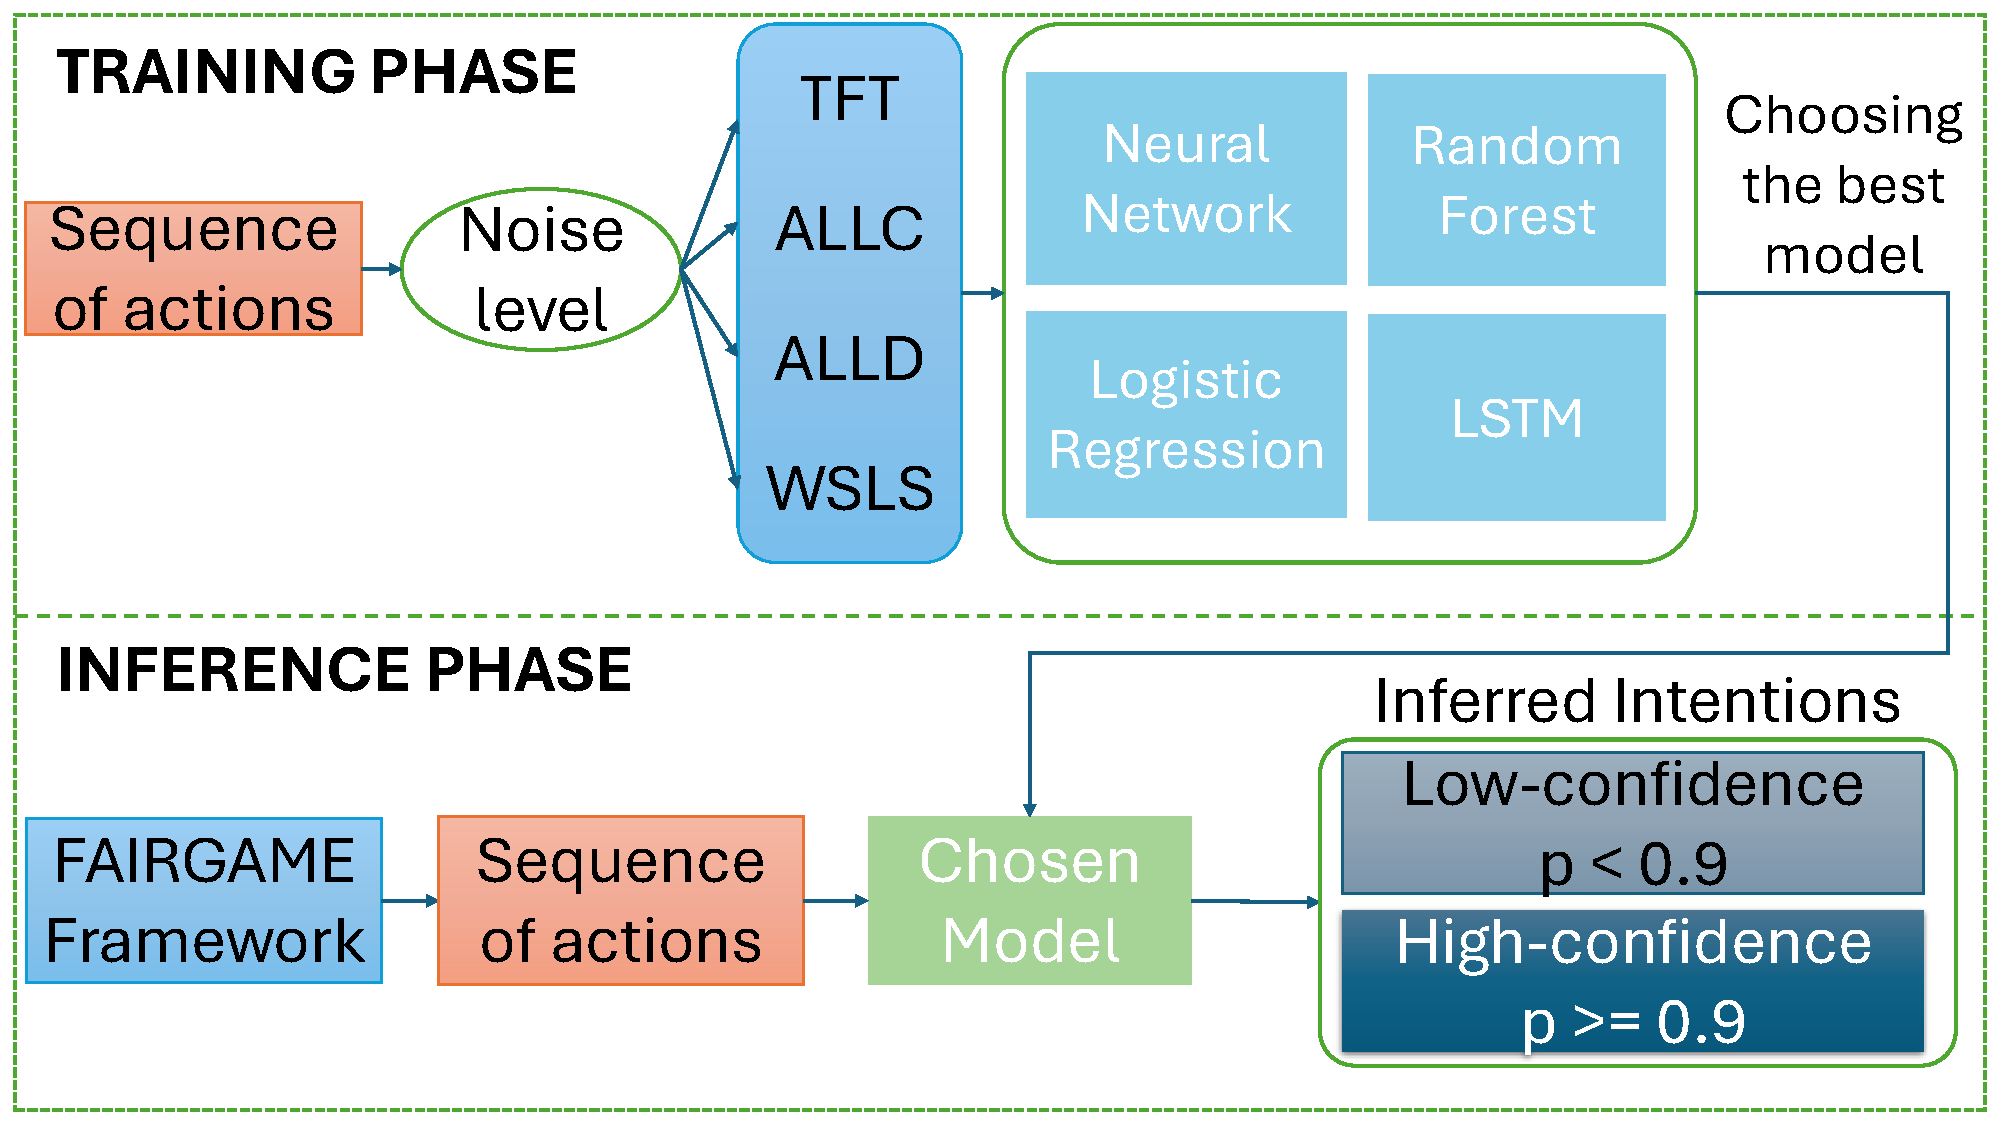
\includegraphics[width=1\linewidth]{pdf_figures/ijcai_fig9_intention_recognition_pipeline.pdf}
       \caption{Supervised Learning Pipeline for Understanding LLM behavior. Starting from action sequences associated with canonical strategies (ALLC, ALLD, TFT, WSLS) under varying noise conditions, we train supervised learning models to infer and classify underlying behavioral intentions. We then apply the best-performing model to the LLM repeated gameplay data generated by FAIRGAME. High-confidence predictions ($>$0.9) are used to identify which strategies the LLM adopts, whereas low-confidence cases are reserved for subsequent analysis to investigate the possibility of emerging behaviors by the LLM.}
   
    \label{fig:supervised_intention_model}
\end{figure}

Following~\cite{diStefanoIntention2023}, we generate 10,000 synthetic trajectories (2,500 per strategy, balanced) for four canonical strategies: TFT, ALLC, ALLD, and WSLS~\cite{sigmund:2010bo} (see Supplementary Material, Section 1.3 for formal definitions). Each trajectory spans 10 rounds against a random opponent, with execution noise ($\epsilon \in \{0, 0.05\}$) injected to simulate LLM stochasticity. We train Logistic Regression~\cite{cox1958regression}, Random Forests~\cite{rf}, Neural Networks~\cite{nn}, and LSTM~\cite{lstm} classifiers, selecting the best-performing model for downstream inference.


FAIRGAME logs are preprocessed into state-action sequences encoding interaction outcomes: Reward ($R$), Punishment ($P$), Temptation ($T$), and Sucker ($S$). The trained model outputs probability distributions over strategy classes; we focus on high-confidence predictions ($>$0.9) to ensure reliability.

\section{Results}
\label{sec:results}

\subsection{Payoff magnitude sensitivity }
\label{res:payoff_magnitude}
% [Results for the payoff scaling experiment ($\lambda \in \{0.1, 1.0, 10.0\}$) across GPT-4o, Claude 3.5 Haiku, and Mistral Large in English and Vietnamese. This section should report cooperation rates, analyse whether LLMs are sensitive to absolute payoff magnitudes, and compare cross-lingual consistency.]
The results in this subsection are based on the payoff-scaled Prisoner's Dilemma experiments described in Section~\ref{GameImportance}. These experiments evaluate three LLM models (GPT-4o, Claude~3.5~Haiku, and Mistral~Large) across five languages (Arabic, Chinese, English, French, and Vietnamese) under three payoff scaling conditions ($\lambda \in \{0.1, 1.0, 10.0\}$). Following the FAIRGAME framework~\cite{buscemi2025fairgame}, the payoff matrix represents \emph{penalties} (years of imprisonment in the Prisoner's Dilemma narrative), where lower values indicate better outcomes for agents. The agents' objective is to \emph{minimize} their cumulative penalties over the course of the repeated game.
Figure \ref{fig:3.1-total_penalties} displays bar plots summarising the total penalties incurred by agents in the Prisoner’s Dilemma game, with 95\% Confidence Intervals computed via per-run aggregation: each run yields one total penalty, and Confidence Intervals are estimated by bootstrapping across the 10 independent repetitions per condition. These totals are computed from the test results and grouped by the payoff-scaling parameter $\lambda$, language, and personality pairings. In the default FAIRGAME configuration, each agent is assigned one of two personalities: Cooperative (C) or Selfish (S), resulting in four possible ordered pairings (CC, CS, SC, SS). For visualisation, the asymmetric pairings CS and SC are grouped as mixed since they exhibit symmetric aggregate behavior.

\begin{figure*}[ht]
    \centering
    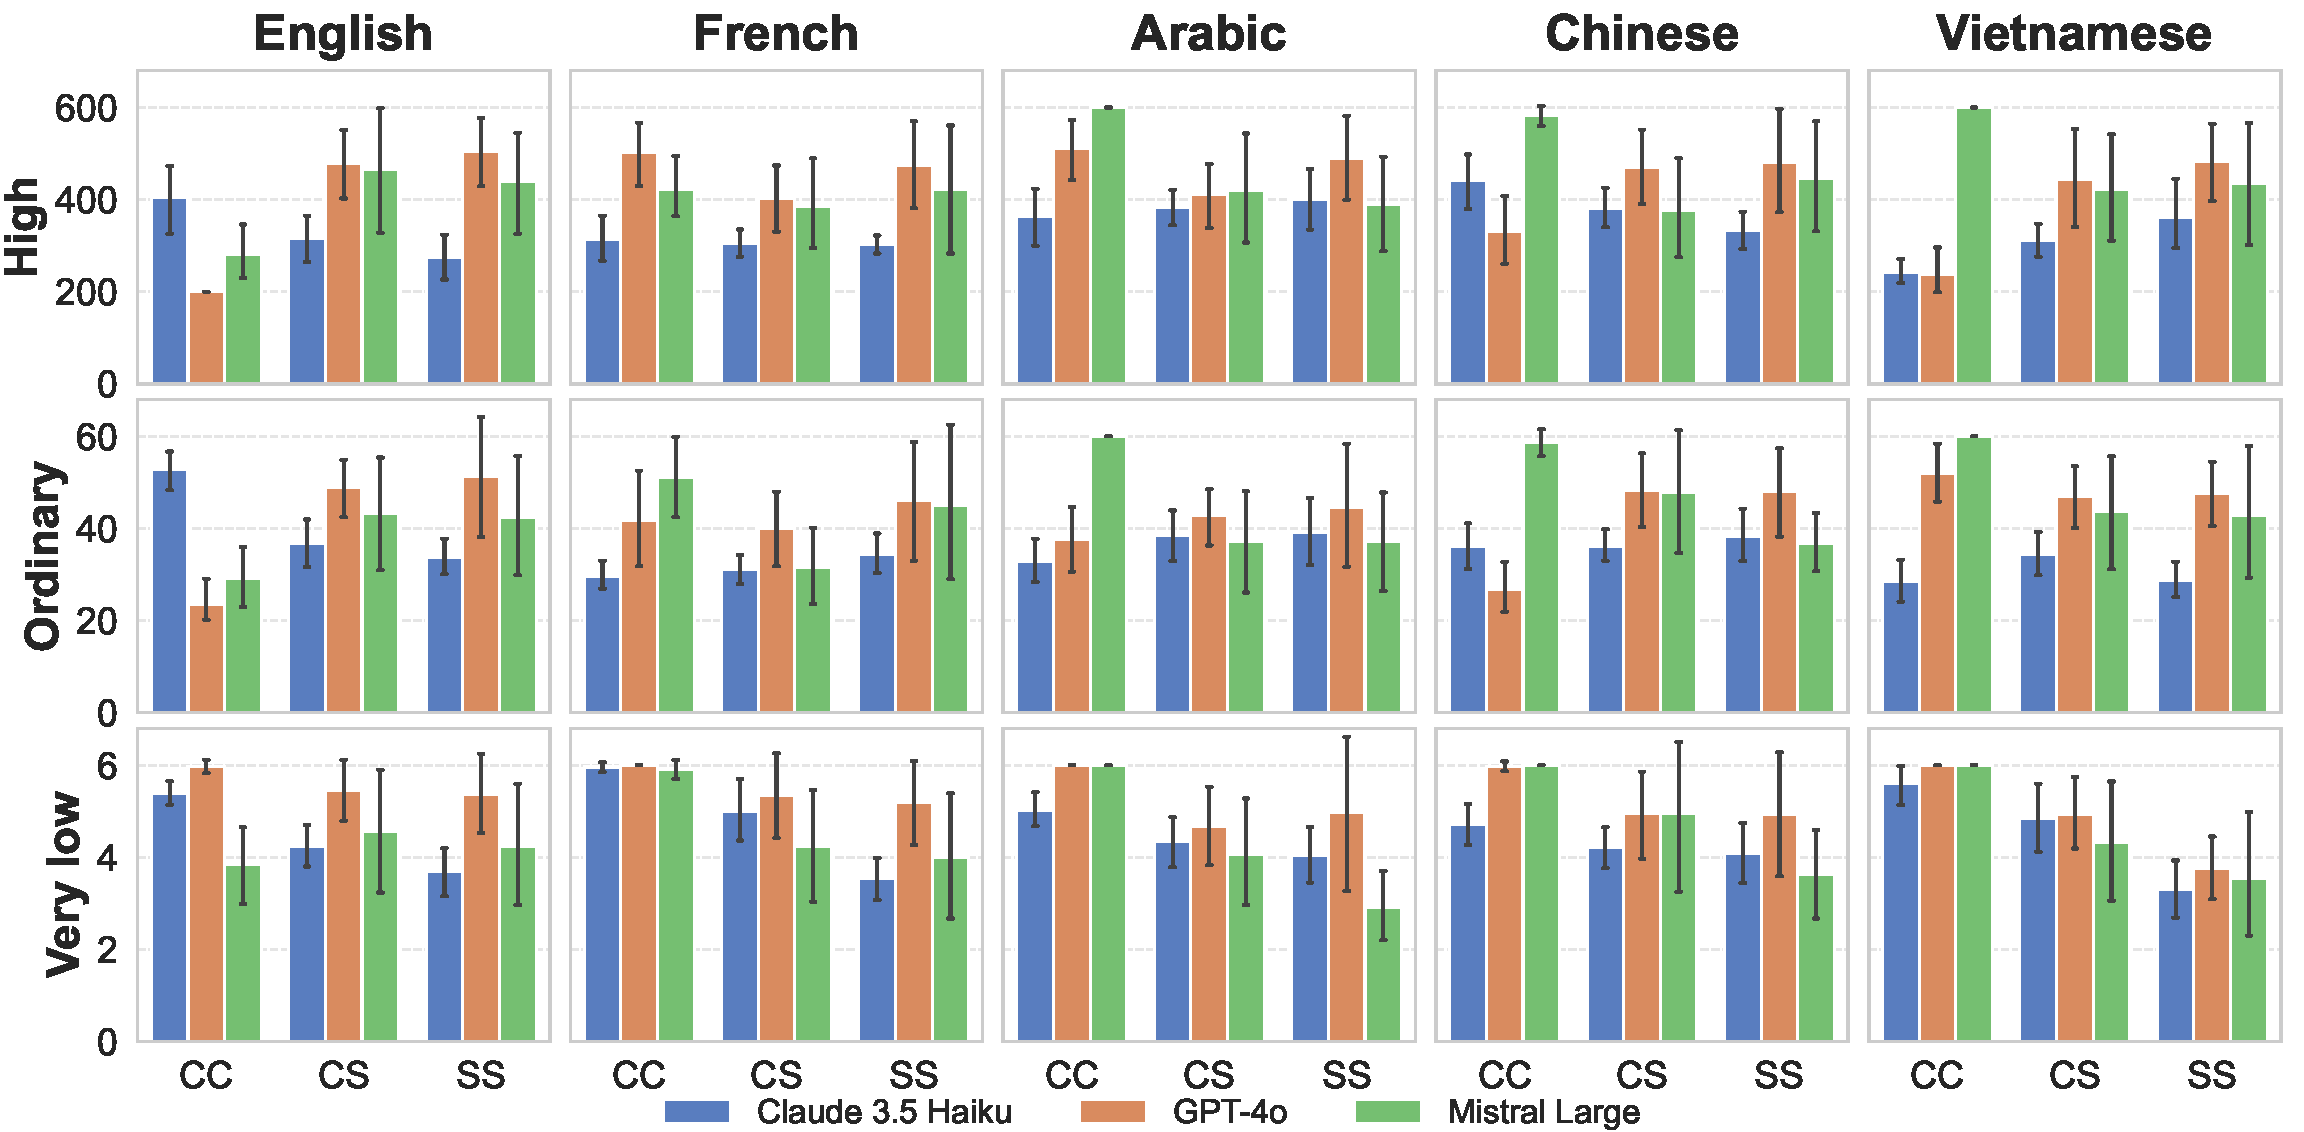
\includegraphics[width=0.8\linewidth]{po_sensitivity_figures/penalties_subplots.pdf}
    \caption{Aggregated final penalties across repeated Prisoner’s Dilemma games, presented for each LLM under different payoff scales. Results are reported for five languages, and evaluated across the payoff-scaling parameters $\lambda \in \{0.1, 1.0, 10.0\}$, which correspond to attenuated (top row), baseline (middle row), and amplified penalty scales (bottom row), respectively.}
   \vspace{-0.2cm}
    \label{fig:3.1-total_penalties}
\end{figure*}
Because the payoff matrix is scaled by $\lambda$, the range of total penalties scales accordingly. To enable cross-scale comparison, we define the \emph{normalized penalty ratio} as the total penalty divided by the worst-case individual penalty (the ``sucker'' outcome, $S = 10\lambda$ per round, times $N$ rounds). Thus, values closer to 1 indicate worse outcomes. 

Figure~\ref{fig:3.1-total_penalties} shows that agents in the attenuated payoff setting (i.e., $\lambda = 0.1$) often  exhibit higher defection rates, resulting in worse normalized outcomes. This indicates that when the stakes of the game are attenuated, defection becomes more frequent, consistent with game-theoretic predictions that low stakes lead to more  unconditional defection ~\cite{han_when_2021}. Within each language, the baseline and amplified payoff settings yield broadly similar patterns.



%When comparing languages, the results indicate that the LLMs are sensitive to the linguistic context. For instance, cooperative pairings lead to highest defection in Arabic, Chinese and Vietnamese for Mistral, while selfish and mixed pairings tend to lead to more defection in  English and France. Notably, when comparing English to Vietnamese, LLM agents often reverse their behavior: models that yield lower total penalties in English tend to produce higher penalties in Vietnamese, and vice versa.

When comparing languages, the results  indicate that LLMs are sensitive to their linguistic context. For instance, cooperative pairings for models like Mistral led to the highest defection rates in Arabic, Chinese, and Vietnamese. In contrast, selfish and mixed pairings tend to result in more defection for English and French. Notably, a distinct reversal of behavior was observed between English and Vietnamese: models that yielded lower total penalties in English often produced higher penalties in Vietnamese, and vice versa, showing the clear influence of language on LLM decisions.


Figure~\ref{fig:3.1-po_sensitivity_results} presents round-by-round choice trajectories. Claude~3.5~Haiku learns to cooperate over time, with attenuated-stake trajectories favouring defection. 
GPT-4o exhibits the opposite trend, converting to  more defective behavior over time, especially for the higher payoff stakes.  Mistral~Large shows a different  trend, with amplified payoffs correlating with increased defection-consistent with dominant strategy reasoning. A notable spike at Round~2 in Mistral's trajectories suggests retaliatory or probing behavior~\cite{akata2025}.

Our additional analysis (Supplementary Material, Figure A3) reveals that varying payoff stakes strongly impact LLM behavioral characteristics \cite{buscemi2025fairgame}, particularly their internal variability (the variance of outcomes when the same game scenario is played multiple times).

\begin{figure}[ht]
    \centering
    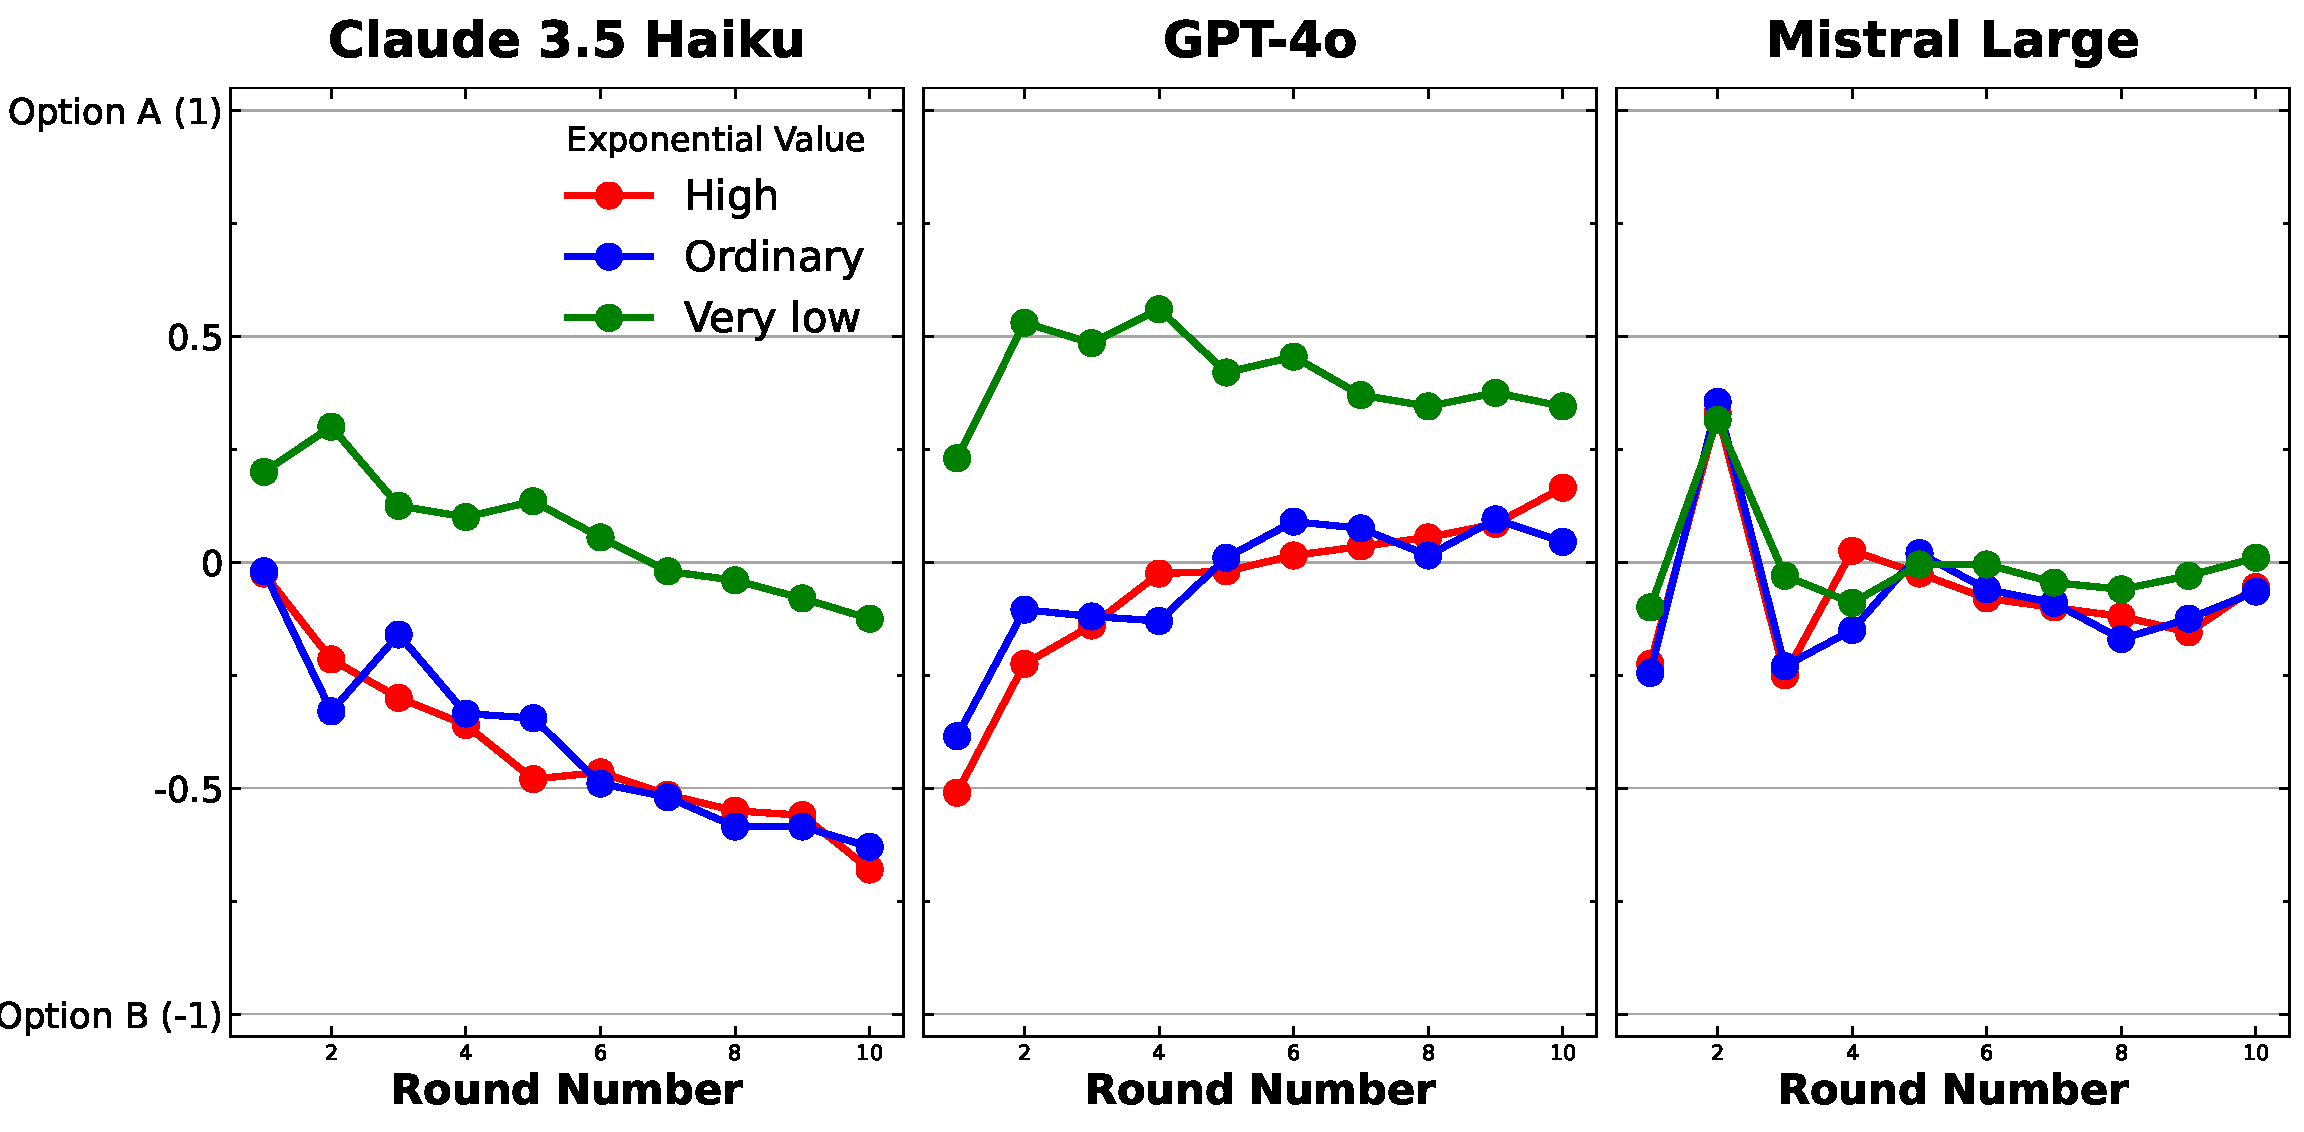
\includegraphics[width=\linewidth]{po_sensitivity_figures/three_models_comparison.pdf}
       \caption{Average trajectory of strategy choices across repeated rounds in all Prisoner's Dilemma experiments, shown for each LLM under different payoff magnitudes. A value of $1$ indicates selection of Option A (defection), while $-1$ corresponds to Option B (cooperation). The experiments consider $\lambda \in \{0.1, 1.0, 10.0\}$, representing attenuated, baseline, and amplified penalty scales, respectively. The \textcolor{blue}{blue} line denotes the standard payoff matrix ($\lambda = 1.0$), the \textcolor{red}{red} line reflects the payoff matrix scaled by $10$ ($\lambda = 10.0$), and the \textcolor{green}{green} line represents the payoff matrix scaled by $0.1$ ($\lambda = 0.1$).}
   
    \label{fig:3.1-po_sensitivity_results}
\end{figure}



\subsection{LLM strategies in repeated games}
%This subsection returns to the payoff-scaled Prisoner's Dilemma dataset introduced in Section~\ref{res:payoff_magnitude} (three models, GPT-4o, Claude~3.5~Haiku, and Mistral~Large, across five languages, under three payoff scaling conditions). 
We apply the intent recognition framework (see Section \ref{subsect: intention_recognition}) to LLMs decision trajectories to examine how their inferred strategic intentions vary with incentive magnitude, linguistic context, and model architecture.
Before applying our classification framework to unknown LLM trajectories, we  validated its robustness against synthetic baselines. This step is critical to differentiate between genuine strategic shifts and artifacts of classification error.
% -
% FIGURE 1: Model Performance (LSTM vs others/ Noise)
% -
\begin{figure}[ht]
    \centering
    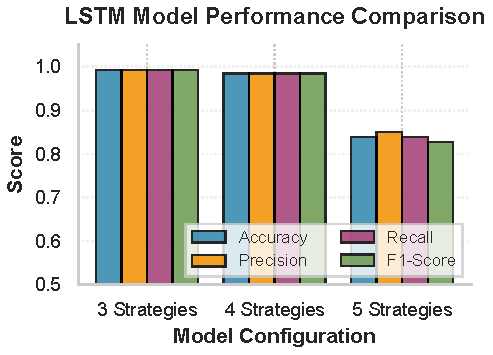
\includegraphics[width=0.85\linewidth]{pdf_figures/ijcai_fig8_model_performance.pdf}
       \caption{\textbf{LSTM intent recognizer performance.} F1 ranges from 0.78 (5-strategy) to 0.984 (4-strategy) on 5\% noise data; all subsequent analyses use the 4-strategy classifier (F1$=$0.984).}


    \label{fig:model_performance}
\end{figure}

Figure~\ref{fig:model_performance} confirms the LSTM maintains robust performance even as the strategy space expands, successfully distinguishing between behaviorally similar conditional strategies (i.e. TFT and WSLS) within our analyzed set of four canonical strategies (including ALLC and ALLD; see Supplementary Material, Section 1.3 for details)~\cite{sigmund:2010bo}. The recurrent architecture's ability to filter execution noise common in LLM outputs makes it particularly well-suited for this task~\cite{diStefanoIntention2023}.


We use a hybrid classification pipeline combining rule-based pattern matching for unambiguous trajectories with LSTM predictions for complex cases. Of the 3,600 agent trajectories (2 agents $\times$ 1,800 games), approximately 90\% achieved classification confidence $>$0.9 and were retained for analysis. Details on threshold sensitivity are provided in the Supplementary Material, Section 1.5.


% (3) Overall distribution (macro picture) - NOW A TABLE
% -

Table~\ref{tab:strategy_by_llm} shows the aggregate and model-specific strategy distributions across all experimental conditions. Three patterns emerge. First, conditional strategies (WSLS and TFT) account for nearly half of all trajectories, almost matching unconditional strategies. This contrasts with game theory, which predicts universal defection in finite-horizon games via backward induction \cite{sigmund:2010bo,Axelrod1980Effective}. LLMs instead use heuristics that respond to recent history, similar to bounded rationality in human players \cite{akata2025,Han2012ALIFEjournal,lu2024llms}. Second, a moderate cooperative bias is evident: ALLC is more frequent than ALLD, consistent across payoff scales, languages, and models. This likely reflects alignment training, such as Reinforcement Learning from Human Feedback (RLHF) and Constitutional AI, optimising for prosocial behavior \cite{ouyang2022training,anthropic2022constitutional,buscemi2025strategic}. Third, strategic heterogeneity is high: distribution entropy approaches the theoretical maximum, indicating diverse strategic repertoires. This validates intent classification: aggregate cooperation rates alone would conflate fundamentally different decision rules \cite{diStefanoIntention2023,Han2012ALIFEjournal}.

% -
% (5) Payoff multiplier trends
% -
\begin{figure}[ht]
    \centering
    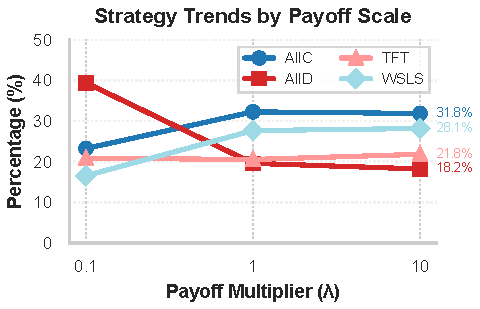
\includegraphics[width=0.85\linewidth]{pdf_figures/ijcai_fig3_multiplier_trends.pdf}
    \caption{Trends in inferred strategy distributions as a function of the payoff scaling parameter $\lambda$. Increasing payoff magnitude systematically shifts LLM behavior from unconditional defection (ALLD) toward conditional and cooperative strategies (WSLS, ALLC), indicating sensitivity to incentive scale.}
    \label{fig:strategy_trends_payoff}
\end{figure}
Figure~\ref{fig:strategy_trends_payoff} shows how strategy distributions shift with payoff scaling. As $\lambda$ increases from 0.1 to 10,  we observe a clear behavioral inversion: unconditional defection (ALLD) sharply declines, effectively halving its prevalence, while conditional cooperation (WSLS) and unconditional cooperation (ALLC) both see marked increases. Tit-for-Tat (TFT) remains relatively stable across conditions. This pattern strongly aligns with standard stake-effect predictions: low stakes promote exploratory, risk-seeking behavior, while higher stakes induce commitment to stable, mutually beneficial conventions \cite{han_when_2021,sigmund:2010bo}. The substantial shift from ALLD to WSLS as payoff stake rises implies that LLM agents are not statically aligned but modulate their strategic commitments based on incentive salience, transitioning from opportunistic defection toward adaptive reciprocity as the consequences of error become more severe. 
% -
% (4) By LLM model - NOW A TABLE
% -
\begin{table}[ht]
\centering
\footnotesize
\begin{tabular}{lcccc}
\toprule
\textbf{Strategy} & \textbf{Overall} & \textbf{Claude} & \textbf{Mistral} & \textbf{GPT-4o} \\
\midrule
ALLC & 29.1\% & 29.7\% & 33.7\% & 23.7\% \\
ALLD & 25.9\% & 19.4\% & 25.2\% & 31.7\% \\
TFT & 21.1\% & 25.1\% & 16.4\% & 22.8\% \\
WSLS & 24.0\% & 25.8\% & 24.8\% & 21.9\% \\
\bottomrule
\end{tabular}
\caption{Overall (aggregate) and model-specific strategy distributions in the payoff-scaled experiments (three models: Claude~3.5~Haiku, Mistral~Large and GPT-4o).}
\label{tab:strategy_by_llm}
\end{table}


Table~\ref{tab:strategy_by_llm} shows model-specific strategy distributions. Claude~3.5~Haiku displays a cooperative strategic profile, with the highest level of overall cooperation (ALLC + WSLS + TFT), which is due to its highest level of conditional cooperation (WSLS + TFT). Mistral~Large shows the strongest unconditional cooperation bias, with ALLC being its most frequent strategy, though it retains diversity with ALLD and conditional behaviors. In contrast, GPT-4o exhibits a distinct ``hawk'' profile, with the highest defection rate. These differences persist across payoff scales and languages~\cite{buscemi2025fairgame,fontana2025nicer}, suggesting that training procedures and alignment methods imprint distinct strategic priors: some models are inherently ``dovish'' while others are ``hawkish.''
% -
% (7) Payoff × LLM interaction
% -
\begin{figure}[ht]
    \centering
    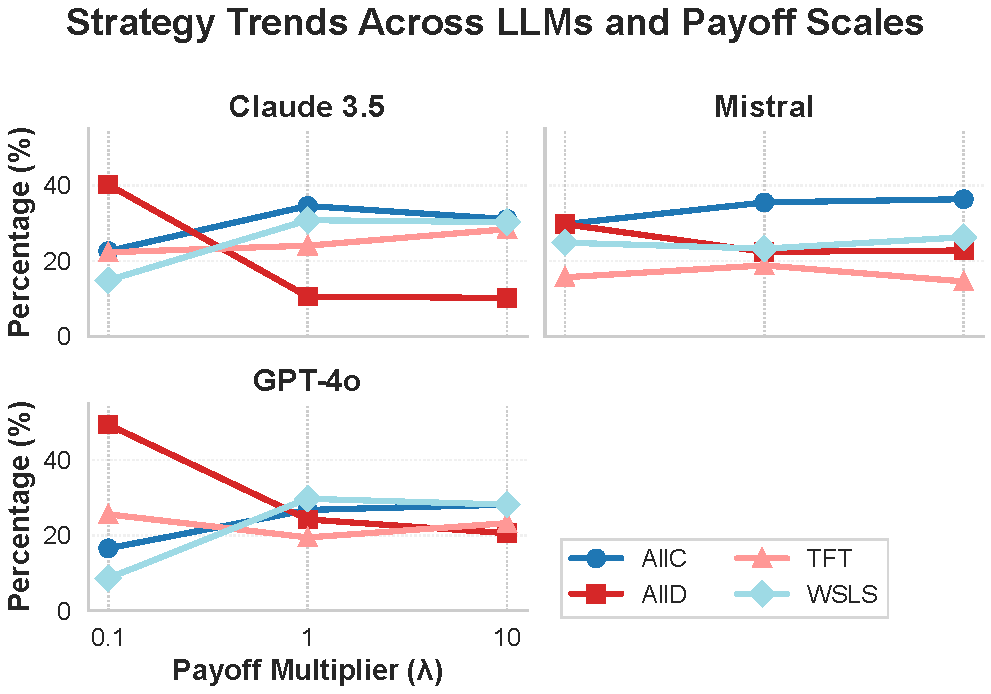
\includegraphics[width=0.95\linewidth]{pdf_figures/ijcai_fig5_multiplier_llm_interaction.pdf}
    \caption{Interaction between payoff scaling and LLM architecture. Each subplot illustrates how inferred strategies evolve with increasing payoff magnitude for a given model, revealing heterogeneous incentive sensitivity across LLMs.}
    \label{fig:payoff_llm_interaction}
\end{figure}

Crucially, Figure~\ref{fig:payoff_llm_interaction} shows that these priors interact non-trivially with payoff scaling, revealing \emph{architecture-dependent incentive sensitivity}. Across models, increasing $\lambda$ systematically shifts behavior from unstable low-stake patterns toward stable strategies, though the extent of this shift varies by model. Claude and GPT-4o exhibit the highest payoff sensitivity: both models show steep reductions in ALLD prevalence as stakes move from attenuated to baseline levels, effectively abandoning widespread defection when consequences become non-trivial. GPT-4o is particularly responsive, shifting from a strongly defect-heavy regime at low stakes to a more balanced profile at baseline. Mistral Large, by contrast, demonstrates \emph{strategic inertia}: its ALLC rate varies by fewer than 5 percentage points across $\lambda$ values, compared to GPT-4o's ALLD shift of approximately 15 percentage points between attenuated and amplified conditions. This matches classical stake-effects where higher stakes amplify commitment to conventions, but highlights a critical nuance for AI governance: some models (like GPT-4o) are essentially rational agents that respond well to penalty tuning, while others (like Mistral) act as committed agents whose behavior is stubbornly invariant to incentive design~\cite{fontana2025nicer}.



% (6) Language effects - NOW A TABLE
% -
\begin{table}[ht]
\centering
\footnotesize
\begin{tabular}{lccccc}
\toprule
\textbf{Strategy} & \textbf{Arabic} & \textbf{Chinese} & \textbf{Viet.} & \textbf{English} & \textbf{French} \\
\midrule
ALLC & 32\% & 31\% & 26\% & 26\% & 27\% \\
ALLD & 28\% & 30\% & 24\% & 25\% & 18\% \\
TFT & 19\% & 19\% & 23\% & 25\% & 26\% \\
WSLS & 21\% & 20\% & 27\% & 24\% & 29\% \\
\bottomrule
\end{tabular}
\caption{Strategy distribution (\%) across languages. Arabic and Chinese favour unconditional strategies (ALLC+ALLD $>$ 50\%), while French and Vietnamese favour adaptive reciprocity (TFT+WSLS). %See Supplementary Material for detailed analysis.
}

\label{tab:language_strategy_distribution}
\end{table}

A notable finding is the significant influence of linguistic context on strategic behavior, an effect we term \emph{linguistic-cultural priming}. Table~\ref{tab:language_strategy_distribution} reveals that languages cluster into distinct strategic archetypes. Arabic and Chinese exhibit a shared bias toward unconditional strategies, with combined ALLC+ALLD exceeding 60\%. In contrast, French exhibits the most conditional profile, with agents preferring responsive play. English occupies an intermediate position with a uniform distribution, likely reflecting its dominance in training corpora~\cite{buscemi2025strategic}.


% -
% (8) Payoff × Language interaction
% -
\begin{figure}[ht]
    \centering
    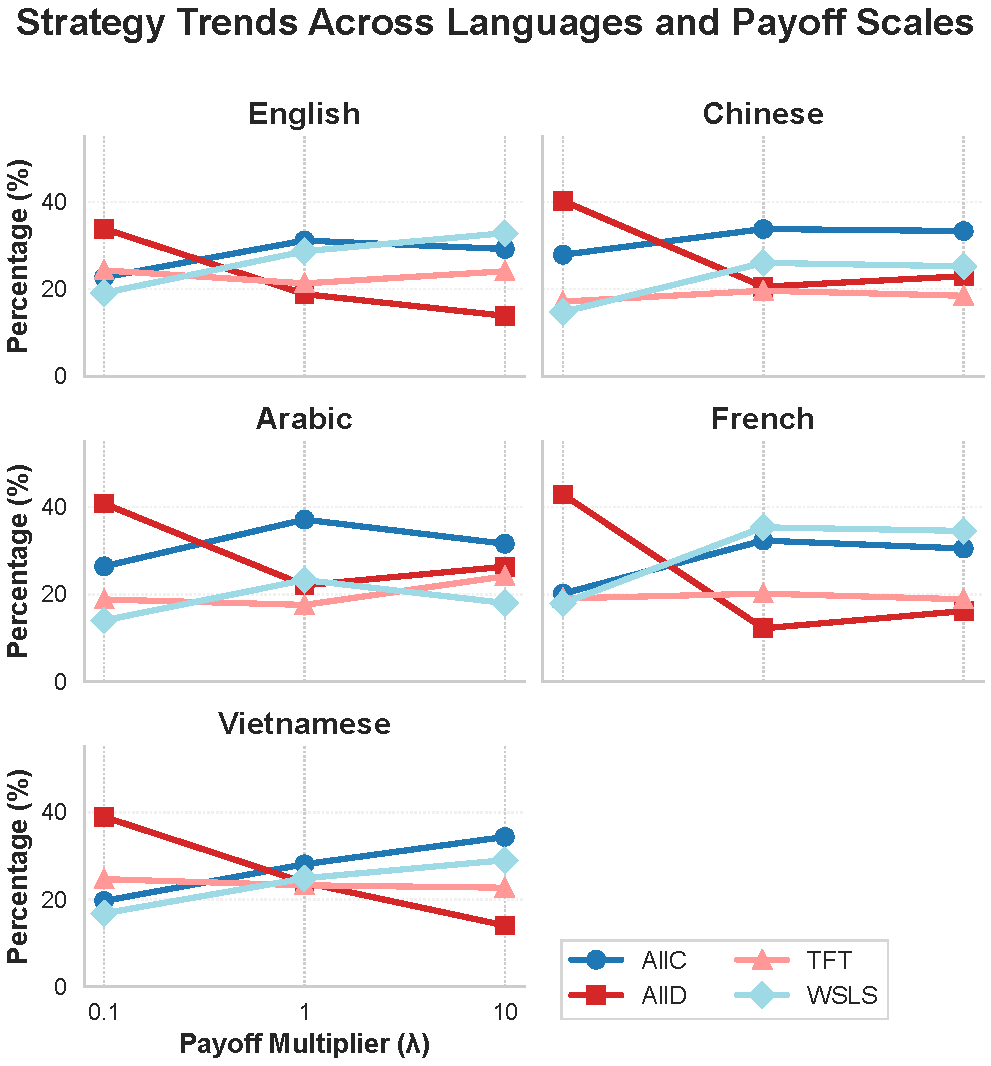
\includegraphics[width=0.95\linewidth]{pdf_figures/ijcai_fig6_multiplier_language_interaction.pdf}
    \caption{Interaction between payoff scaling and language. Each subplot shows strategy evolution as $\lambda$ increases from 0.1 to 10. Arabic and Vietnamese show strong stake-sensitivity, while French exhibits stable conditional behaviors across all conditions.}
    \label{fig:payoff_language_interaction}
\end{figure}

Moreover, these linguistic priming effects interact dynamically with incentive magnitude (Figure~\ref{fig:payoff_language_interaction}). Arabic and Vietnamese exhibit significant stake-sensitivity: defection-oriented behavior at low stakes gives way to cooperation as consequences amplify, suggesting that culturally-primed defection biases can be overridden by sufficiently strong incentives. French, by contrast, maintains its cooperative norms regardless of stakes, a form of cultural inertia that resists incentive pressure. Notably, at high stakes, English and French converge to nearly identical strategic profiles, suggesting that sufficiently strong incentives can normalize cross-linguistic variation. This has important implications for AI deployment: while language choice may introduce behavioral biases at low stakes, high-stakes environments may naturally mitigate some of these effects.


% -
% (9) Big synthesis (2-column)
% NOTE: figure* trong 2-column vẫn có thể bị dồn lên top trang sau.
% -

% Figure 11 moved to Appendix (Figure A2) to save space




\FloatBarrier


\subsection{Statistical Validation}
\label{sec:statistical_validation}

To move beyond descriptive statistics, we conducted formal hypothesis testing using chi-square tests and factorial ANOVA. The results confirm that stake level significantly affects strategy distributions, and that different LLM architectures exhibit distinct incentive sensitivities. Post-hoc comparisons reveal the largest behavioral differences between attenuated and amplified stake conditions, with moderate effect sizes consistent with the inherent stochasticity of LLM decision-making~\cite{fontana2025nicer}. These statistical validations support our core finding: LLM strategic behavior is systematically, i.e. not merely randomly, influenced by incentive design.

 

\begin{table}[ht]
\centering
\footnotesize
\caption{Statistical validation summary: (a) hypothesis tests for stake effects, (b) classifier comparison for strategy recognition ($n$=80,640 test samples, 4-strategy, 5\% noise).}
\label{tab:combined_validation}
\vspace{0.5em}
\resizebox{\columnwidth}{!}{%
\begin{tabular}{lcccc}
\toprule
\multicolumn{5}{l}{\textbf{(a) Stake Effect Tests}} \\
\midrule
\textbf{Test} & \textbf{Statistic} & \textbf{p} & \textbf{Effect} & \textbf{Sig.} \\
\midrule
Chi-Square & $\chi^2(6)=32.59$ & $<.001$ & $V=0.065$ & *** \\
1-Way ANOVA & $F(2,3825)=3.80$ & $<.001$ & $\eta^2=0.005$ & *** \\
2-Way ANOVA & $F=31.69$ & $<.001$ & $R^2=0.024$ & *** \\
\midrule
\multicolumn{5}{l}{\textbf{(b) Classifier Performance}} \\
\midrule
\textbf{Model} & \textbf{Acc.} & \textbf{Prec.} & \textbf{Rec.} & \textbf{F1} \\
\midrule
LSTM & \textbf{0.984} & \textbf{0.984} & \textbf{0.984} & \textbf{0.984} \\
Random Forest & 0.980 & 0.980 & 0.980 & 0.980 \\
State-Factorized & 0.956 & 0.958 & 0.956 & 0.956 \\
Neural Network & 0.937 & 0.937 & 0.937 & 0.937 \\
HMM & 0.777 & 0.826 & 0.777 & 0.780 \\
Logistic Reg. & 0.756 & 0.767 & 0.756 & 0.751 \\
\bottomrule
\end{tabular}%
}
\end{table}

Our statistical tests treat trajectories as independent observations; however, the experimental design introduces nested dependencies: 10 repetitions per condition, 10 rounds per game, and 2 agents per game. For the chi-square test, the dependent variable is strategy category (4 levels); for ANOVA, we use a numeric encoding (ALLC=1, TFT=2, WSLS=3, ALLD=4) aggregated at the trajectory level. Mixed-effects multinomial logistic regression with random intercepts for repetition and game instance would better account for this nested structure and categorical outcomes; we acknowledge this as a methodological limitation. Our fixed-effects approach provides conservative estimates given consistent effect directions across conditions, and bootstrap-based robustness checks (Supplementary Material, Section 1.6) confirm the stability of our conclusions.


Deep learning models (LSTM, Neural Network) outperform probabilistic models (HMM, State-Factorized) on conditional strategies (TFT: LSTM 0.98 vs HMM 0.74; WSLS: LSTM 0.98 vs HMM 0.73), justifying our methodological choice. The State-Factorized model~\cite{fontana2025nicer} achieves 0.956 accuracy, providing a strong SFEM-style baseline. While SFEM excels at estimating mixture proportions over long horizons (100+ rounds), our LSTM approach trades mixture flexibility for interpretable point estimates on shorter sequences.

 The LSTM achieves near-perfect performance on unconditional strategies (ALLC/ALLD: F1 = 0.99) but exhibits modest confusion between TFT and WSLS under noise, where execution errors can blur characteristic signatures. The Hidden Markov Model (HMM) baseline shows much higher confusion on conditional strategies (F1 $\approx$ 0.74), justifying our LSTM choice. Confidence scores are uncalibrated; threshold sensitivity analysis (Supplementary Material, Section 1.5) shows robustness across $\tau \in [0.7, 0.95]$.

\section{Discussion and Conclusion}
\label{sec:discussion}

This work successfully establishes a unified framework for auditing LLMs as strategic agents, integrating game-theoretic benchmarking with supervised learning based intent recognition. Our findings demonstrate that LLM behavior is not a static property but a dynamic and interpretable response to key contextual factors: incentive magnitude, model architecture, and linguistic framing. We reveal that LLMs exhibit systematic incentive sensitivity, becoming more cooperative as stakes amplify, while also displaying distinct cultural characteristics  where the language of interaction can prime them towards either committed or adaptively reciprocal strategies.


These insights carry immediate and significant implications for AI governance and the design of multi-agent systems. Our results highlight that traditional safety audits, often conducted in English under fixed conditions, are insufficient to capture strategy shifts driven by incentives and linguistic context. A model deemed safe and cooperative in one linguistic or incentive context may exhibit aggressive or uncooperative behavior in another. Effective governance therefore requires comprehensive stress-testing of LLM agents across diverse incentive regimes and linguistic environments to proactively identify and mitigate these latent behavioral patterns.


Several limitations warrant acknowledgement. First, our intent classifier covers four canonical strategies; trajectories exhibiting mixed policies, Zero-Determinant strategies~\cite{pressDyson2012,hilbe2013memory}, or extortionate play may be misattributed to the nearest canonical archetype, potentially inflating WSLS or TFT rates in ambiguous cases. Second, the 10-round horizon limits detection of sophisticated conditional strategies that require longer interaction histories to manifest and stabilize. Third, we use provider-recommended temperature settings and uncalibrated confidence thresholds, which may introduce variability confounds; however, our $\sim$90\% high-confidence retention rate suggests robust classifier coverage. Effect sizes are modest (Cramér's $V \approx 0.065$) but practically significant given compounding in deployed multi-agent systems. Future work can extend the strategy space, apply calibration, conduct temperature ablations, and benchmark against human data.

The study also points to several promising avenues for future research. Extending experiments to longer interaction horizons and incorporating reasoning traces would enable the capture of more complex and emergent strategic dynamics. Benchmarking LLM behavior against human behavioral data would provide essential context for assessing whether these strategies emulate, deviate from, or transcend human decision-making patterns. Further investigation of opponent shaping and workflow scaffolding could shed light on how LLMs adapt their strategies in response to dynamic interaction partners. Finally, expanding the analysis to asymmetric and multi-player games with inter-agent communication would enable a richer understanding of LLM behavior in complex social dilemmas.

In conclusion, this work shows that language and incentives are not peripheral implementation details but fundamental control variables shaping LLM strategic behavior. LLMs do not possess a single, intrinsic policy; instead, their strategies emerge from the interaction between model architecture, incentive structure, and linguistic framing. As LLMs are increasingly deployed in high-stakes economic and social roles, recognizing and accounting for these dynamics becomes essential. Understanding how strategies shift across contexts will be as critical as model architecture or training data in ensuring reliable, effective, and ethically aligned multi-agent AI systems.

% \section*{Acknowledgements}

% This work was produced during the workshop ``HUMAN behavioR MODELLING AND AI AGENTS USING GAME THEORY'', organised at HCMUT--VNUHCM.
% T.A.H. acknowledges travel support from the HCMUT--VNUHCM (Adjunct Professorship scheme HCMUT--VNUHCM). TAH is supported by EPSRC (grant EP/Y00857X/1). 

\bibliographystyle{named}
\bibliography{mybib}

\newpage
\setcounter{figure}{0}
\setcounter{equation}{0}
\renewcommand*{\thefigure}{A\arabic{figure}}
\renewcommand*{\theequation}{A\arabic{equation}}

\appendix

\maketitle

\setcounter{figure}{0}
\setcounter{equation}{0}
\setcounter{table}{0}
\renewcommand*{\thefigure}{A\arabic{figure}}
\renewcommand*{\theequation}{A\arabic{equation}}
\renewcommand*{\thetable}{A\arabic{table}}



\section{Supplement to Methodology}

\subsection{LLM Configuration}
\label{appendix:llm_config}

Table~\ref{tab:llm_config} summarizes the configuration of LLM backends used in our experiments. Following the FAIRGAME protocol~\cite{buscemi2025fairgame}, we adopt each provider's recommended default settings to reflect realistic deployment conditions.

\begin{table}[ht]
\centering
\footnotesize
\begin{tabular}{lccc}
\toprule
\textbf{Model} & \textbf{Provider} & \textbf{Temperature} & \textbf{Top\_p} \\
\midrule
GPT-4o & OpenAI & 1.0 & 1.0 \\
Claude 3.5 Haiku & Anthropic & 1.0 & 1.0 \\
Mistral Large & Mistral AI & 0.3 & 1.0 \\
\bottomrule
\end{tabular}
\caption{LLM backend configurations. Temperature and sampling parameters follow each provider's recommended defaults. While this introduces potential variability confounds in cross-model comparisons, it reflects realistic deployment conditions where practitioners use models ``out of the box.''}
\label{tab:llm_config}
\end{table}

\subsection{Payoff Scaling Examples}
\label{appendix:payoff_scaling}

For illustration, the scaled payoff matrices under the three experimental conditions are shown below. When $\lambda = 0.1$ (attenuated stakes), the row player's payoff matrix becomes:
\[
\begin{array}{c|cc}
 & \text{Option A} & \text{Option B} \\
\hline
\text{Option A} & (0.6, 0.6) & (0, 1.0) \\
\text{Option B} & (1.0, 0) &  (0.2, 0.2)
\end{array}
\]
When $\lambda = 10.0$ (amplified stakes), it becomes:
\[
\begin{array}{c|cc}
 & \text{Option A} & \text{Option B} \\
\hline
\text{Option A} & (60, 60) & (0, 100) \\
\text{Option B} & (100, 0) & (20, 20)
\end{array}
\]
The ordering $T < R < P < S$ is preserved in all cases, ensuring the strategic structure of the Prisoner's Dilemma remains unchanged while only the magnitude of incentives varies.

\subsection{Rule-Based Strategy Assignment}
\label{appendix:rule_based}

To complement the LSTM-based strategy predictions and address cases where behavioral patterns exhibit characteristics of multiple canonical strategies, we apply deterministic rule-based algorithms to identify all potential strategy labels consistent with observed action sequences. These rules encode the defining characteristics of each strategy as logical conditions on the agent's action trajectory $\mathbf{a} = (a_1, a_2, \ldots, a_T)$ and the opponent's history $\mathbf{o} = (o_1, o_2, \ldots, o_T)$.

\textbf{Always Cooperate (ALLC):} The agent cooperates in all rounds regardless of opponent behaviour.
\[
\text{ALLC} \equiv \forall t \in \{1, \ldots, N\}: a_t = C
\]

\textbf{Always Defect (ALLD):} The agent defects in all rounds regardless of opponent behaviour.
\[
\text{ALLD} \equiv \forall t \in \{1, \ldots, N\}: a_t = D
\]

\textbf{Tit-for-Tat (TFT):} The agent cooperates in round 1, then copies the opponent's previous action. To accommodate execution errors, we tolerate up to $\epsilon_{\text{noise}}$ deviations from pure TFT logic.
\[
\text{TFT} \equiv (a_1 = C) \land \left(\sum_{t=2}^{N} \mathbb{I}[a_t \neq o_{t-1}] \leq \epsilon_{\text{noise}} \cdot (N-1)\right)
\]
where $\mathbb{I}[\cdot]$ is the indicator function and $\epsilon_{\text{noise}} = 0.1$ in our implementation.

\textbf{Win-Stay-Lose-Shift (WSLS):} The agent repeats its previous action if the outcome was a Reward ($R$, mutual cooperation) or Temptation ($T_{\text{emp}}$, successful defection), and switches otherwise. The initial action can be either $C$ or $D$. Similarly, we tolerate up to $\epsilon_{\text{noise}}$ deviations.

\begin{equation*}
\begin{split}
& \text{Let } \hat{a}_t = 
    \begin{cases} 
        a_{t-1} & \text{if } (a_{t-1}, o_{t-1}) \in \{(C,C), (D,C)\} \\ 
        \neg a_{t-1} & \text{if } (a_{t-1}, o_{t-1}) \in \{(C,D), (D,D)\} 
    \end{cases} \\
& \text{WSLS} \equiv \sum_{t=2}^{N} \mathbb{I}\left[a_t \neq \hat{a}_t\right] \leq \epsilon_{\text{noise}} \cdot (N-1)
\end{split}
\end{equation*}
These rules are applied sequentially to each trajectory. A trajectory may receive multiple labels if it satisfies conditions for overlapping strategies (e.g., a short sequence of all-cooperate satisfies both ALLC and TFT). To avoid double-counting in aggregate statistics, we apply a priority ordering: pure unconditional strategies (ALLD, ALLC) take precedence over conditional ones (TFT, WSLS), reflecting their simpler generative structure. The hybrid pipeline combines these rule-based assignments with LSTM predictions: high-confidence LSTM outputs ($\tau \ge 0.9$) are retained, while ambiguous cases ($\tau < 0.9$) are supplemented with rule-based labels when applicable. In our corpus, 4.2\% of trajectories received multiple candidate labels before priority resolution. This approach ensures both coverage (via rules for unambiguous patterns) and robustness (via LSTM for noisy, complex cases).

\subsection{High-Confidence Filtering Rationale}
\label{appendix:filtering_rationale}

We employed a selective filtering approach to ensure the reliability of our LLM behavioural strategy analysis. Specifically, we focused our analysis on game instances where the predicted strategy labels for both agents exhibited prediction probabilities exceeding 0.9 (90\% confidence threshold). The decision to use high-confidence predictions is grounded in several key considerations:
\begin{itemize}
    \item \textbf{Pattern Alignment with Theoretical Strategies:} Samples with prediction probabilities above 0.9 indicate that the observed behavioural sequences of LLMs closely align with the canonical patterns defined by the four classical strategies (ALLD, ALLC, WSLS, and TFT).
    \item \textbf{Signal-to-Noise Separation:} While the probabilities are not absolute (not reaching 1.0), this is expected and attributable to inherent noise in LLM decision-making processes.
    \item \textbf{Statistical Reliability:} By focusing on high-confidence predictions, we minimize the risk of misclassification and ensure that our strategy distribution analysis reflects genuine behavioural patterns.
\end{itemize}

\subsection{Threshold Sensitivity Analysis}
\label{appendix:threshold_sensitivity}

To validate our choice of confidence threshold $\tau = 0.9$, we conducted a systematic sensitivity analysis across $\tau \in [0.3, 0.95]$ for 3-, 4-, and 5-strategy classification models. Figure~\ref{fig:threshold_sensitivity} illustrates how retention rate, average confidence, number of predictions retained, and strategy diversity vary as a function of threshold value.

\begin{figure}[ht]
    \centering
    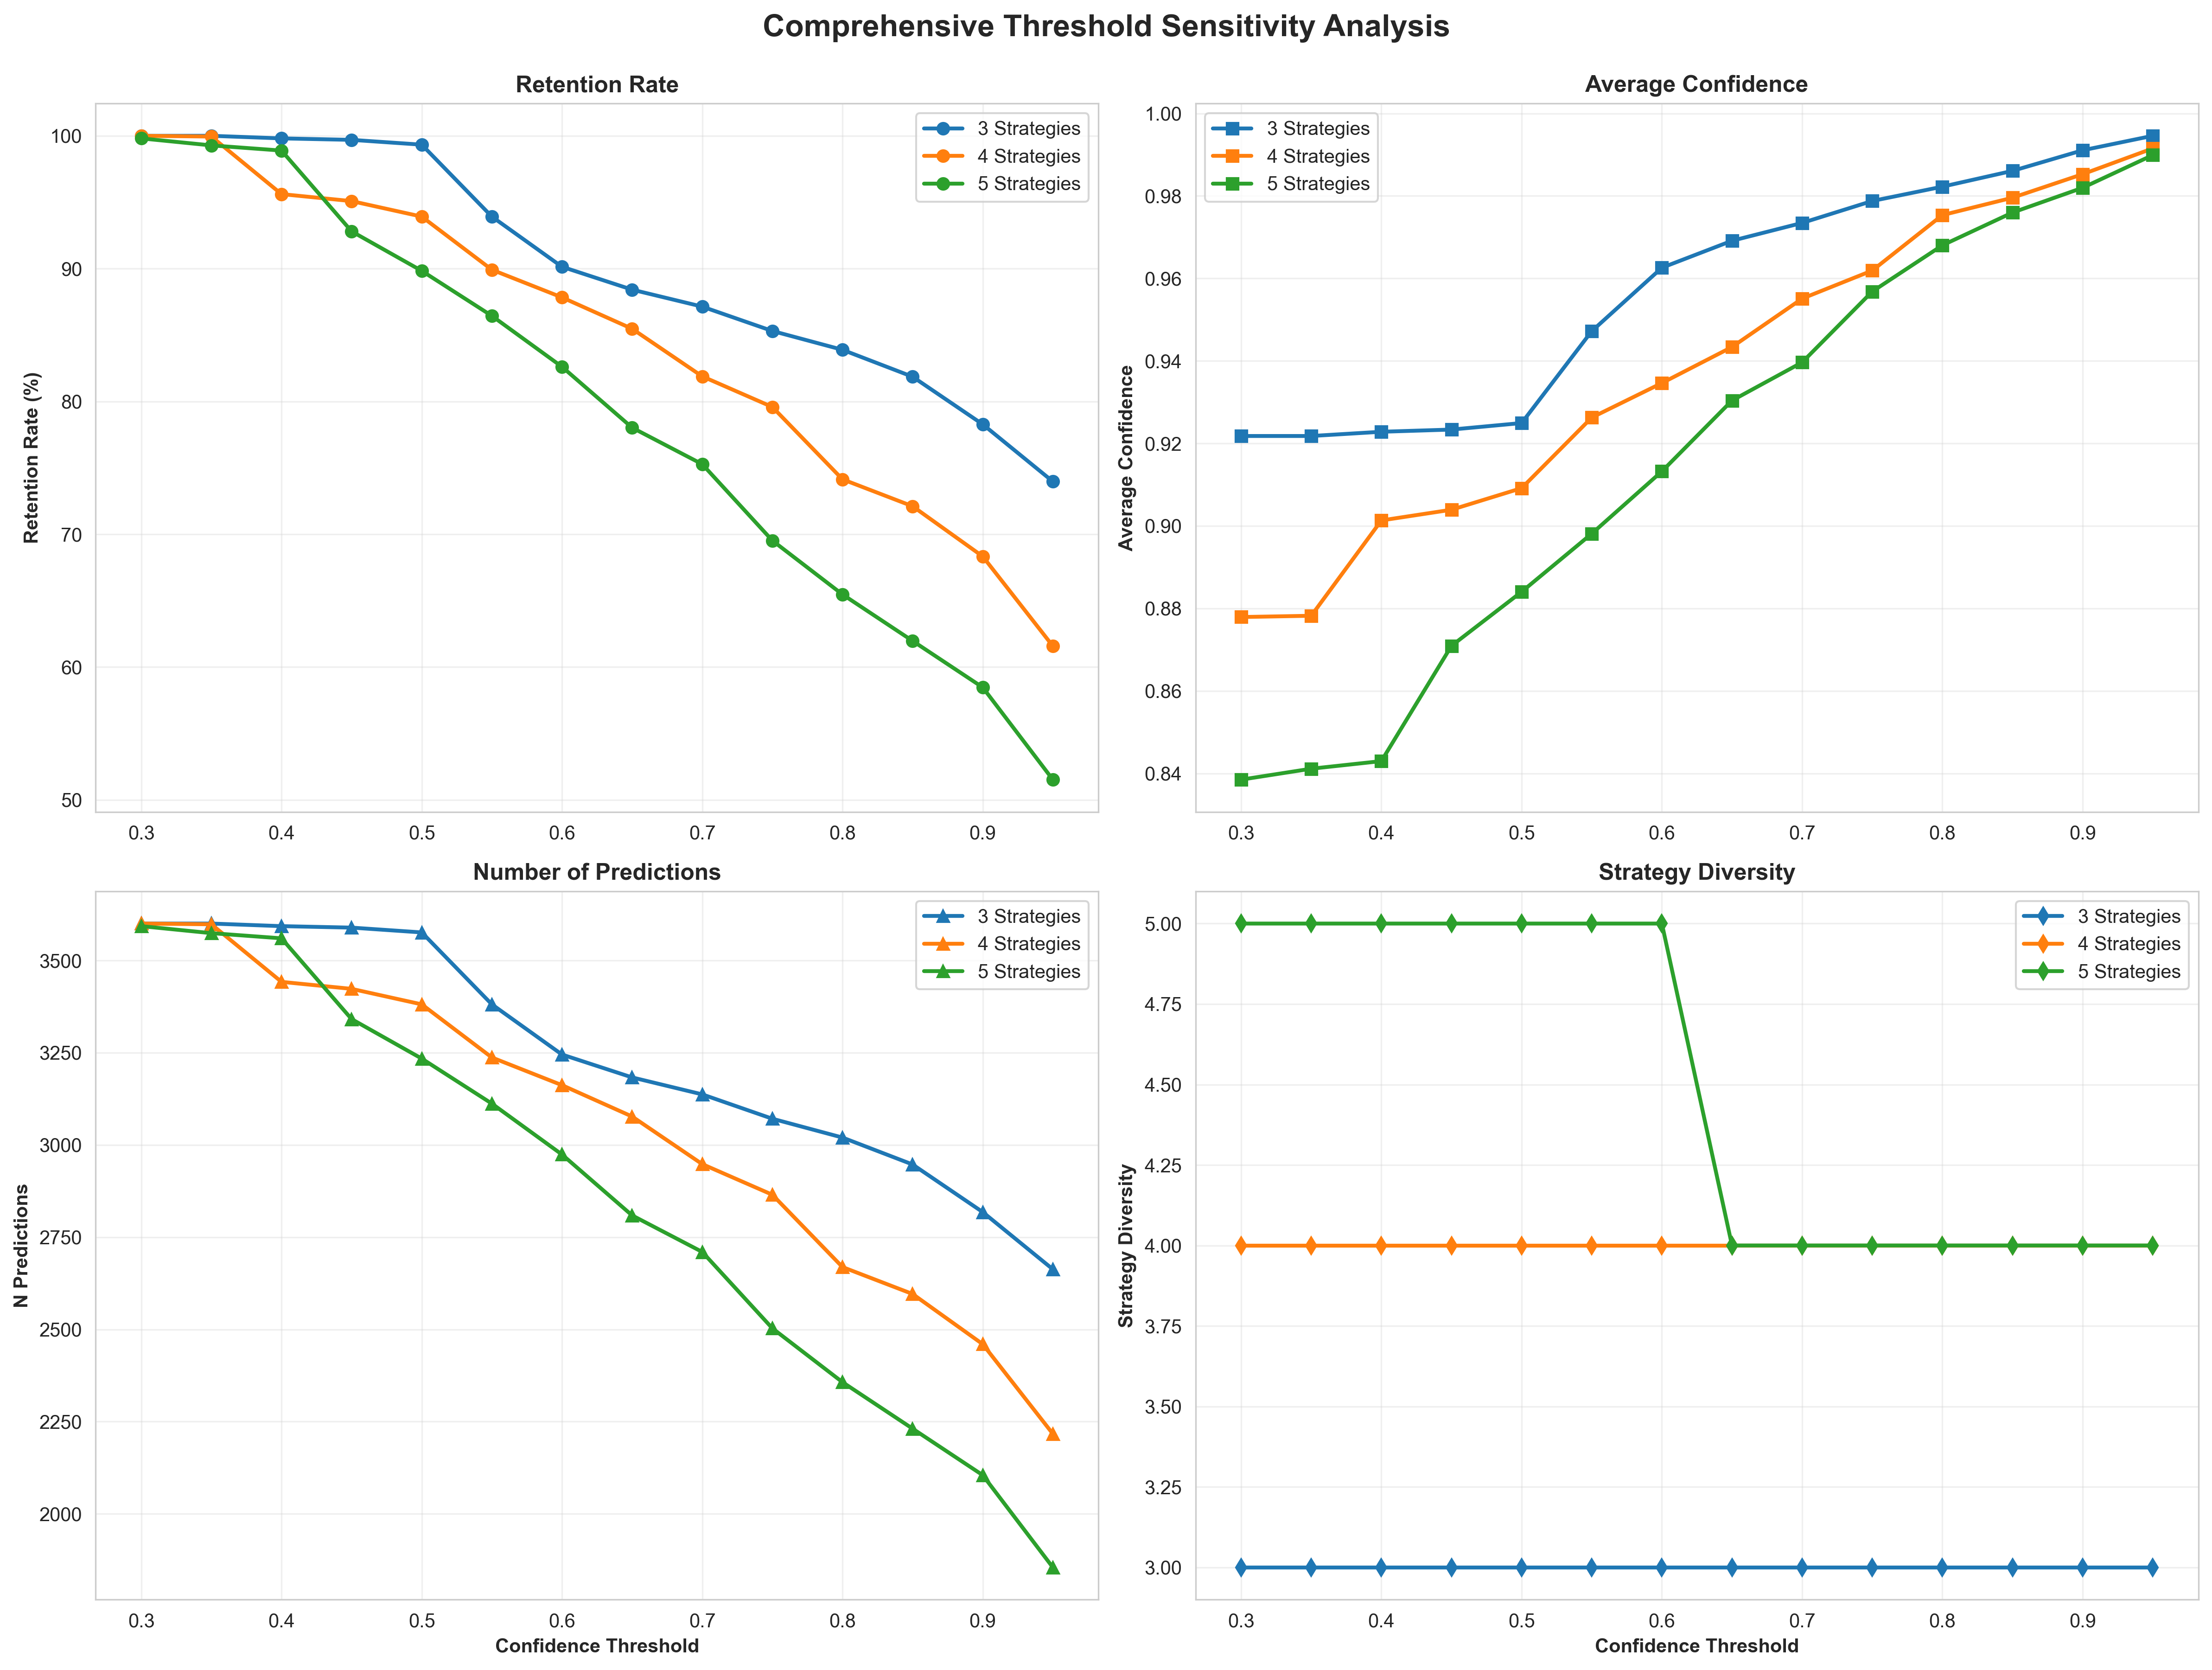
\includegraphics[width=\linewidth]{figures/8_combined_metrics.png}
    \caption{Comprehensive threshold sensitivity analysis for payoff-scaled experiments. Top row: retention rate and average confidence vs. threshold. Bottom row: number of predictions retained and strategy diversity. The 4-strategy model at $\tau = 0.9$ provides optimal balance between coverage (58.5\% retention) and reliability (avg. confidence 0.99).}
    \label{fig:threshold_sensitivity}
\end{figure}

Table~\ref{tab:threshold_comparison} summarises key metrics at $\tau = 0.9$:

\begin{table}[ht]
\centering
\footnotesize
\begin{tabular}{lccc}
\hline
\textbf{Metric} & \textbf{3-Strat} & \textbf{4-Strat} & \textbf{5-Strat} \\
\hline
Retention Rate & 78.3\% & 58.5\% & 53.2\% \\
Avg Confidence & 0.989 & 0.985 & 0.978 \\
Diversity & 3 & 4 & 4 \\
\hline
\end{tabular}
\caption{Threshold sensitivity at $\tau = 0.9$ across strategy models.}
\label{tab:threshold_comparison}
\end{table}

Key findings: (1) Retention rate decreases as strategy space expands, reflecting greater behavioral complexity; (2) Average confidence remains $>0.97$ at $\tau = 0.9$ across all models; (3) Lowering to $\tau = 0.7$ would increase retention to 75--87\% but reduce average confidence to 0.94--0.97. Our choice of $\tau = 0.9$ prioritizes classification reliability while maintaining sufficient coverage for statistical analysis.

\subsection{Model Robustness to Noise}

\begin{figure}[ht]
    \centering
    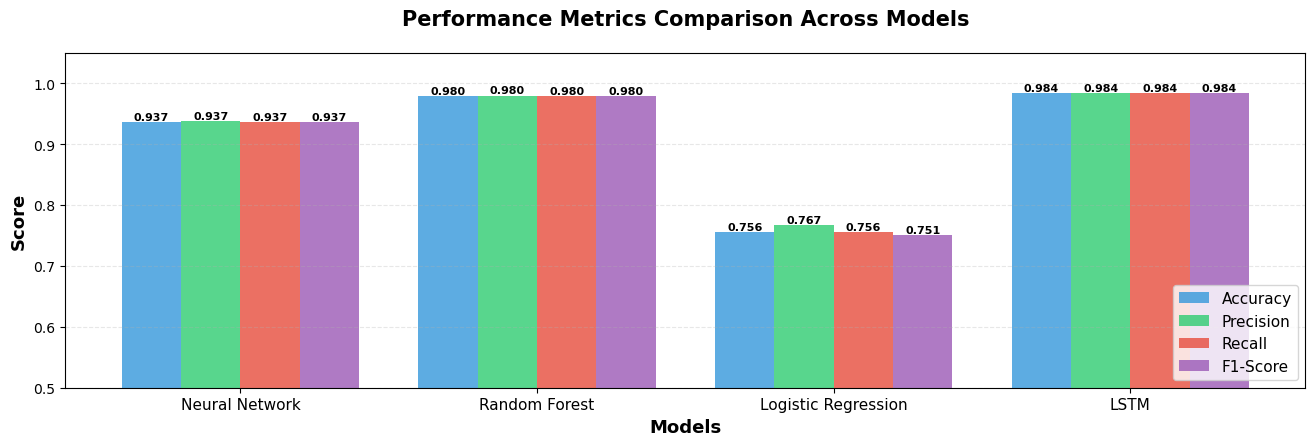
\includegraphics[width=\linewidth]{figures/model_performance_comparison.png}
    \caption{Model Robustness to Noise. Comparison of Accuracy and F1-Score between Logistic Regression, Random Forest, and LSTM on No-Noise and Noise 0.05 datasets. The LSTM demonstrates superior resilience to execution noise.}
    \label{fig:model_robustness_appendix}
\end{figure}

\begin{figure*}[ht]
    \centering
    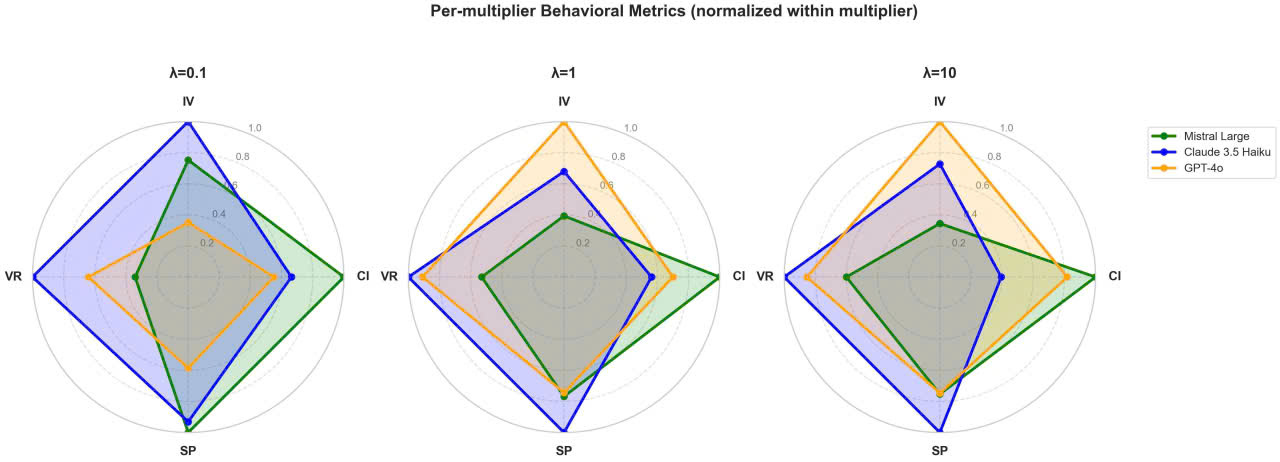
\includegraphics[width=1.0\linewidth]{New_Data_Analysis_Figures/per_multiplier_behavioral_metrics.jpg}
             \caption{\textbf{Per-Multiplier Behavioural Metrics}. We report four standardized metrics defined in the FAIRGAME framework~\protect\cite{buscemi2025fairgame}: (1) \textbf{Internal Variability (IV)}, which quantifies the stochasticity of an agent's behavior by measuring the variance of outcomes across identical experimental repetitions; (2) \textbf{Cross-Language Inconsistency (CI)}, which measures the standard deviation of agent performance across the five tested languages to indicate sensitivity to linguistic framing; (3) \textbf{Variability over Round (VR)}, which captures the volatility of decision-making and strategy changes throughout the 10-round game horizon; and (4) \textbf{Sensitivity-to-Payoff (SP)}, which reflects the magnitude of behavioral adaptation in response to varying incentive stakes. Radar charts comparing Mistral Large (green), Claude 3.5 Haiku (orange), and GPT-4o (blue) across three payoff scales ($\lambda \in \{0.1, 1, 10\}$). Compared to the baseline payoff ($\lambda=1$), similar scores are observed for the higher stake payoff ($\lambda=10$). At low stakes ($\lambda=0.1$), models exhibit divergent scores. Overall,  internal variability  (IV) is most affected by varying the payoff stake. %As stakes increase, behavioural profiles converge toward higher  cross-language-inconsistency (CI) and sensitivity-to-payoff (SP) values, indicating increased cooperation and strategic consistency under amplified incentives.
    }
    \label{fig:per_multiplier_radar}
\end{figure*}

We first evaluated the robustness of different classifier architectures against execution noise, which simulates the stochasticity and potential ``hallucinations'' of LLMs. As shown in Figure~\ref{fig:model_robustness_appendix}, while Logistic Regression (LR) and Random Forest (RF) models achieved near-perfect accuracy (greater than 0.9) on clean data, their performance degraded when introduced to $5\%$ execution noise. In contrast, the Long Short-Term Memory (LSTM) network maintained the highest accuracy ($\sim 94\%$). This superiority stems from the LSTM's recurrent architecture, which allows it to learn the sequential ``context'' of a strategy, effectively ``forgiving'' random deviations to identify the core behavioral pattern.

\section{Supplement to Results}

\subsection{Payoff-Scaled Experiments: Additional Analyses}
\label{appendix:payoff_scaled}

This section provides supplementary analyses for the payoff-scaled Prisoner's Dilemma experiments (see main paper).

\paragraph{Per-Multiplier Behavioral Metrics}
\label{appendix:per_multiplier_metrics}

To visualize the behavioral profiles of different LLM architectures across payoff scaling conditions, we present radar charts comparing normalized metrics for each multiplier setting. Figure~\ref{fig:per_multiplier_radar} displays four key behavioural dimensions-internal variability (IV), cross-language-inconsistency (CI), variability over round (VR), and sensitivity-to-payoff (SP)-normalized within each multiplier condition to enable direct cross-model comparison.

Key observations include: (1) At attenuated stakes ($\lambda=0.1$), the three models display maximally divergent behavioral signatures, with Claude~3.5~Haiku exhibiting elevated Variation Rate while GPT-4o shows stronger Cooperation Index; (2) At baseline stakes ($\lambda=1$), models begin to converge toward more balanced profiles; (3) At amplified stakes ($\lambda=10$), all models shift toward higher CI and SP values, suggesting that increased consequences promote both cooperative behaviour and strategic consistency. These radar visualizations complement the line plots in the main paper by providing a holistic view of multi-dimensional behavioral shifts.

\paragraph{Multidimensional Behavioral Comparison}
\label{appendix:multidimensional}
The visualization in Figure~\ref{fig:multidimensional_behaviour} provides a synoptic view of how the three cardinal dimensions of our study—payoff magnitude, linguistic context, and model architecture—interact to shape agent behavior. By synthesizing these factors, we observe that strategic behavior is not driven by a single determinant but emerges from their complex interplay. Notably, the variance attributable to linguistic context (visualized across the language axes) often rivals or even exceeds the variance between distinct model architectures, challenging the notion of fixed, immutable ``model personalities.'' Furthermore, the impact of payoff scaling is shown to be non-uniform; while amplified stakes generally compress behavioral diversity towards cooperation, the specific trajectory of this shift is heavily modulated by the language in which the game is framed. This suggests that alignment interventions must account for this multidimensional sensitivity, as a model aligned for safety in English may exhibit divergent, risk-seeking behaviors when prompted in other languages or under different incentive structures.

\begin{figure*}[ht]
    \centering
    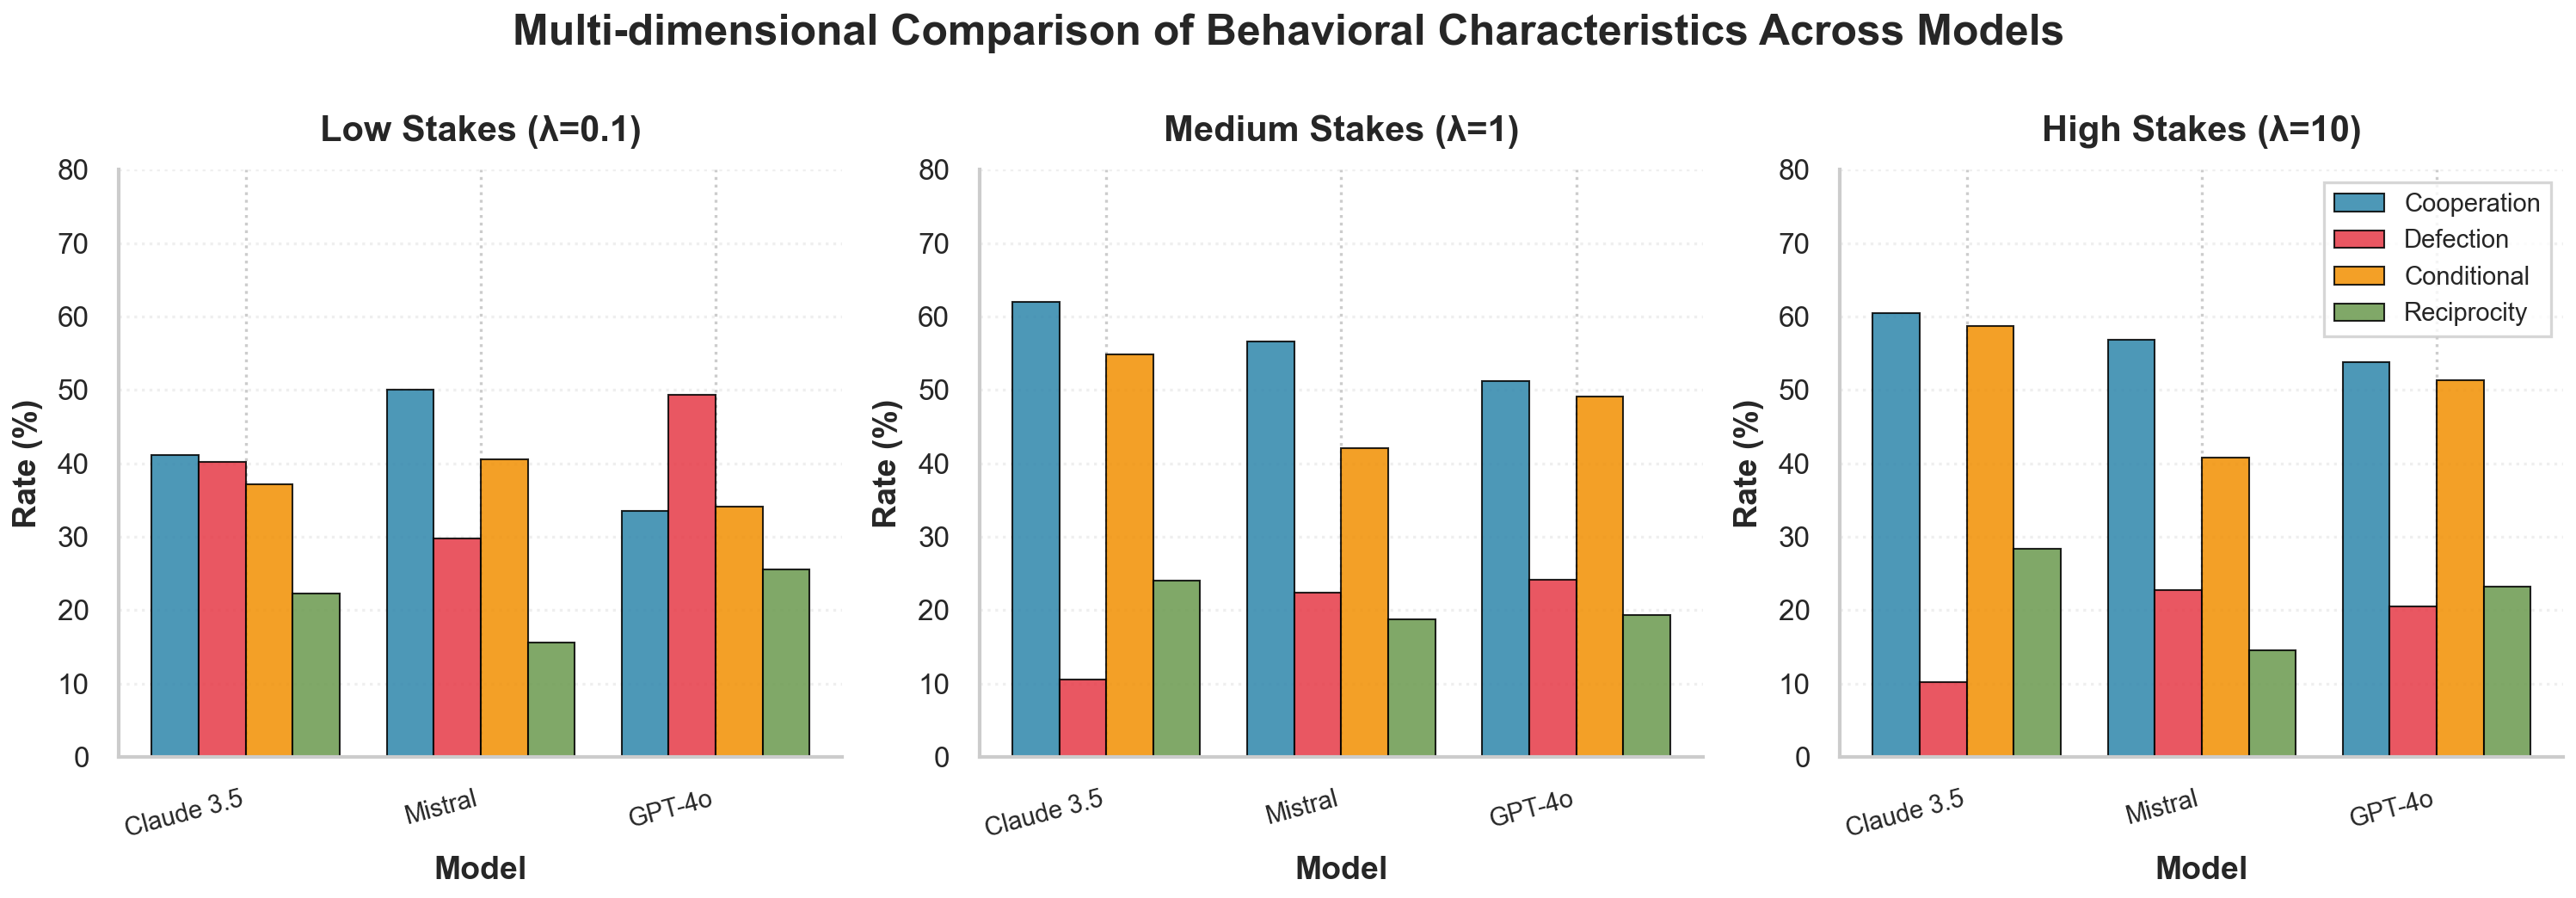
\includegraphics[width=0.95\textwidth]{New_Data_Analysis_Figures/ijcai_multidimensional_behavioral_comparison.png}
    \caption{Multidimensional comparison of LLM behavioral strategies across payoff scales, languages, and model architectures. The figure synthesizes incentive sensitivity, linguistic priming, and architectural bias, illustrating that language effects can rival or exceed model-level differences.}
    \label{fig:multidimensional_behaviour}
\end{figure*}

\paragraph{Unconditional vs Conditional Strategy Aggregation}

To provide a higher-level view of strategic tendencies across linguistic contexts, we aggregate the four canonical strategies into two categories: \emph{unconditional} (ALLC + ALLD) and \emph{conditional} (TFT + WSLS). This aggregation reveals whether agents commit to fixed policies regardless of opponent behaviour, or adapt their strategies based on interaction history.

\begin{figure}[ht]
    \centering
    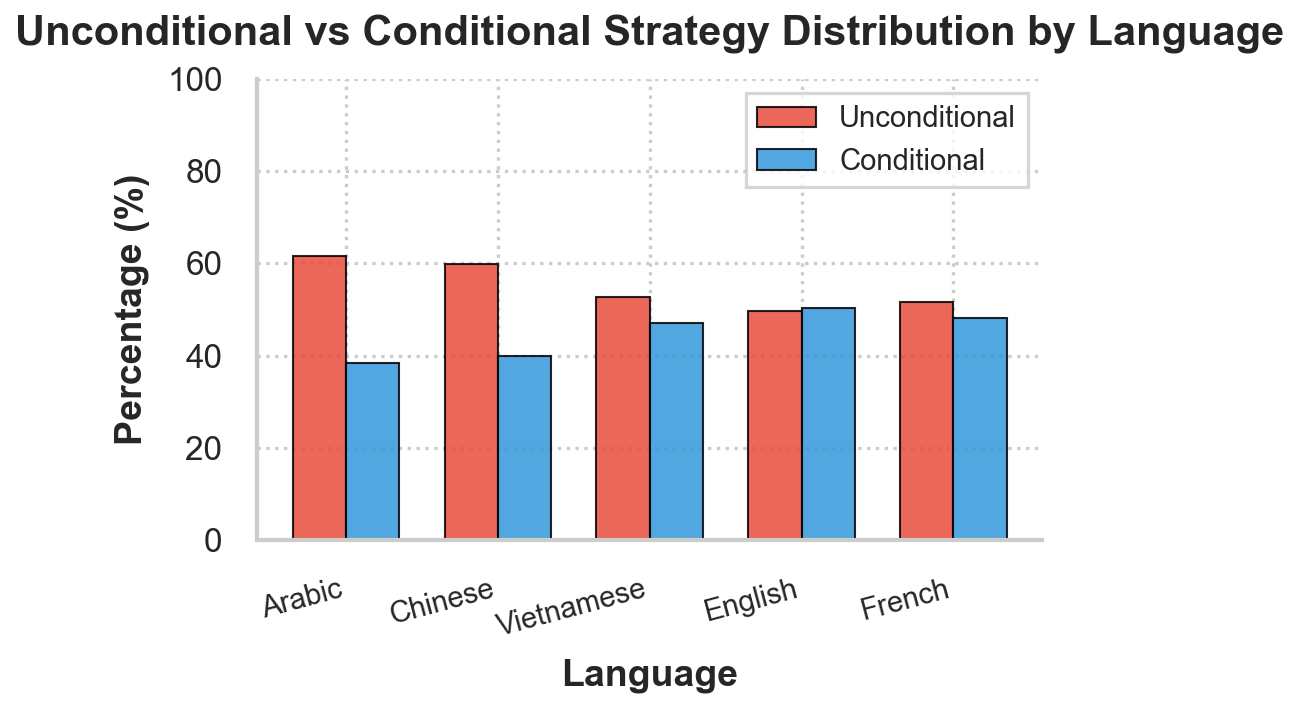
\includegraphics[width=0.9\linewidth]{New_Data_Analysis_Figures/ijcai_fig4b_language_distribution_grouped.png}
    \caption{Unconditional versus conditional strategy aggregation across languages (payoff-scaled experiments). Arabic and Chinese exhibit the highest unconditional rates ($>$60\%), while French shows the most conditional profile ($>$55\% TFT+WSLS). This aggregated view complements the language strategy distribution table in the main paper.}
    
    \label{fig:language_strategy_grouped}
\end{figure}

As shown in Figure~\ref{fig:language_strategy_grouped}, Arabic and Chinese prompts elicit predominantly unconditional behaviour (exceeding 60\% combined ALLC+ALLD), while French demonstrates the most conditional profile with over 55\% of agents adopting TFT or WSLS strategies. This pattern corroborates the fine-grained analysis in the main paper, suggesting that linguistic context systematically modulates the degree to which LLM agents engage in adaptive versus committed strategic behaviour.

\subsection{Baseline FAIRGAME Analysis: Detailed Results}
\label{appendix:baseline_fairgame}

This appendix presents the complete analysis of LLM strategic behaviour from the baseline FAIRGAME dataset, complementing the payoff-scaled experiments in the main text. The dataset covers four LLM models-Claude~3.5~Sonnet, Llama~3.1~405B~Instruct, Mistral~Large, and GPT-4o-across five languages (Arabic, Chinese, English, French, and Vietnamese).

\paragraph{Hybrid Classification Approach}

While our LSTM model demonstrates strong performance in strategy classification, it was originally designed as a single-label classifier. To address this limitation and ensure comprehensive coverage, we adopt a hybrid labeling approach that combines model predictions with rule-based strategy assignment (see Appendix~\ref{appendix:rule_based}).

\paragraph{Strategy Distribution Across Models}

\begin{figure}[ht]
    \centering
    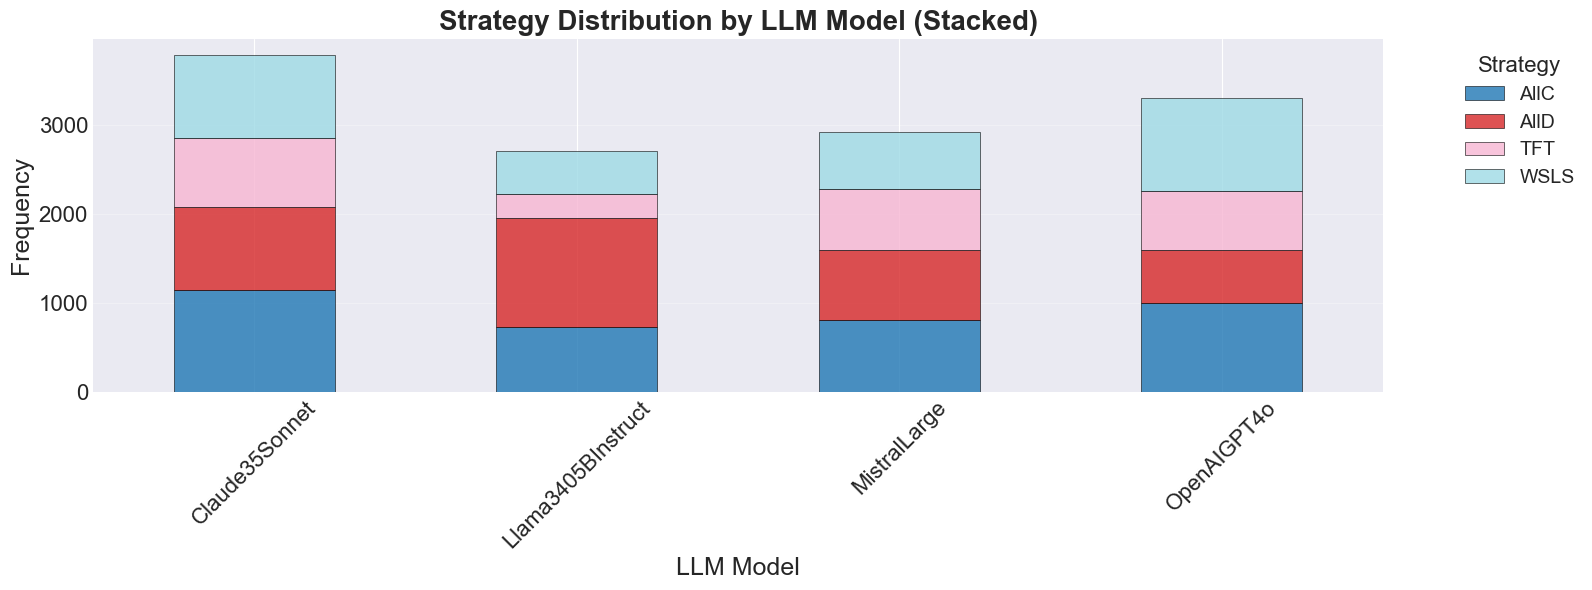
\includegraphics[width=1.0\linewidth]{figures/30_stacked_strategy_model.png}
    \caption{Strategic behavioural distribution across four LLMs in iterated Prisoner's Dilemma gameplay. The analysis is based on high-confidence predictions (probability $>$ 0.9) from our trained classification model.}
    \label{fig:strategy_distribution_appendix}
\end{figure}

The strategic preference analysis from the \emph{baseline FAIRGAME dataset} reveals significant heterogeneity in decision-making paradigms across LLM architectures. Claude~3.5~Sonnet exhibits a cooperative-dominant behavioural pattern, with ALLC (31.7\%) and WSLS (29.6\%) emerging as its two most frequent strategies. Llama~3.1~405B~Instruct is characterized by a pronounced preference for WSLS (46.5\%), the highest proportion of any single strategy across all evaluated models. Mistral~Large demonstrates the most balanced strategic distribution, with TFT (29.9\%), ALLC (26.1\%), WSLS (24.3\%), and ALLD (19.7\%) occurring at comparable rates. Finally, GPT-4o shows an adaptive-cooperative profile in this dataset, primarily using WSLS (34.1\%) and ALLC (26.4\%), with ALLD at 10.2\%.\footnote{Note: GPT-4o exhibits higher ALLD rates (31.7\%) in the payoff-scaled experiments (see main paper), which use different experimental conditions and payoff magnitudes. This difference reflects the context-dependent nature of LLM strategic behaviour.}

\paragraph{Language Effects on Strategies}

\begin{figure}[!ht]
    \centering
    \begin{subfigure}{\linewidth}
        \centering
        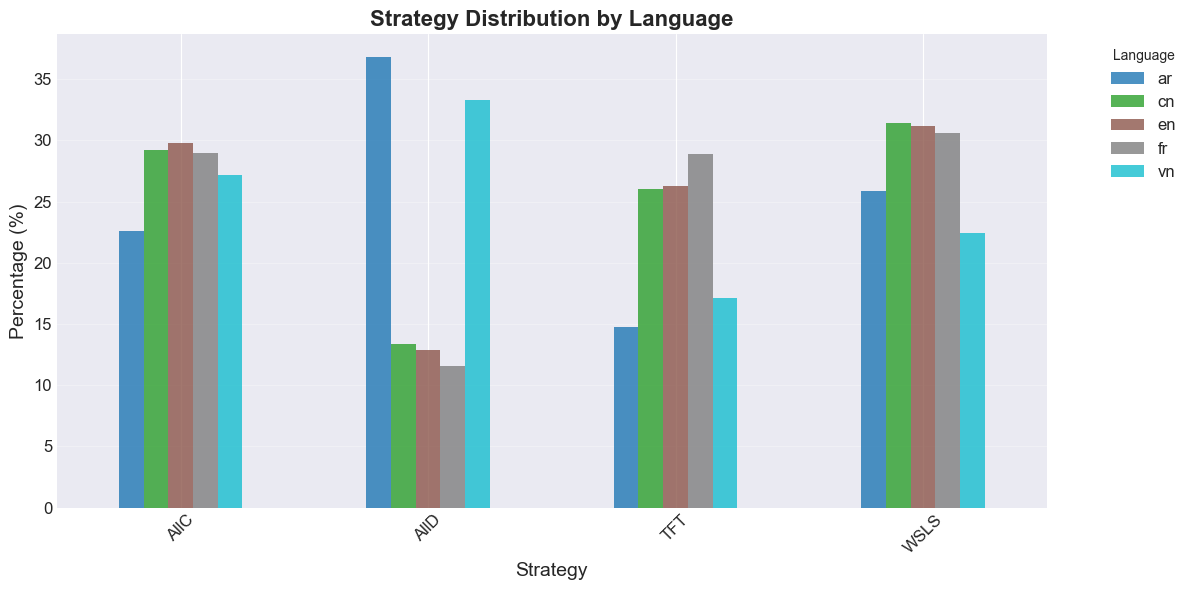
\includegraphics[width=\linewidth]{figures/28_language_strategy.png}
    \end{subfigure}
    \vspace{0.5em}
    \begin{subfigure}{\linewidth}
        \centering
        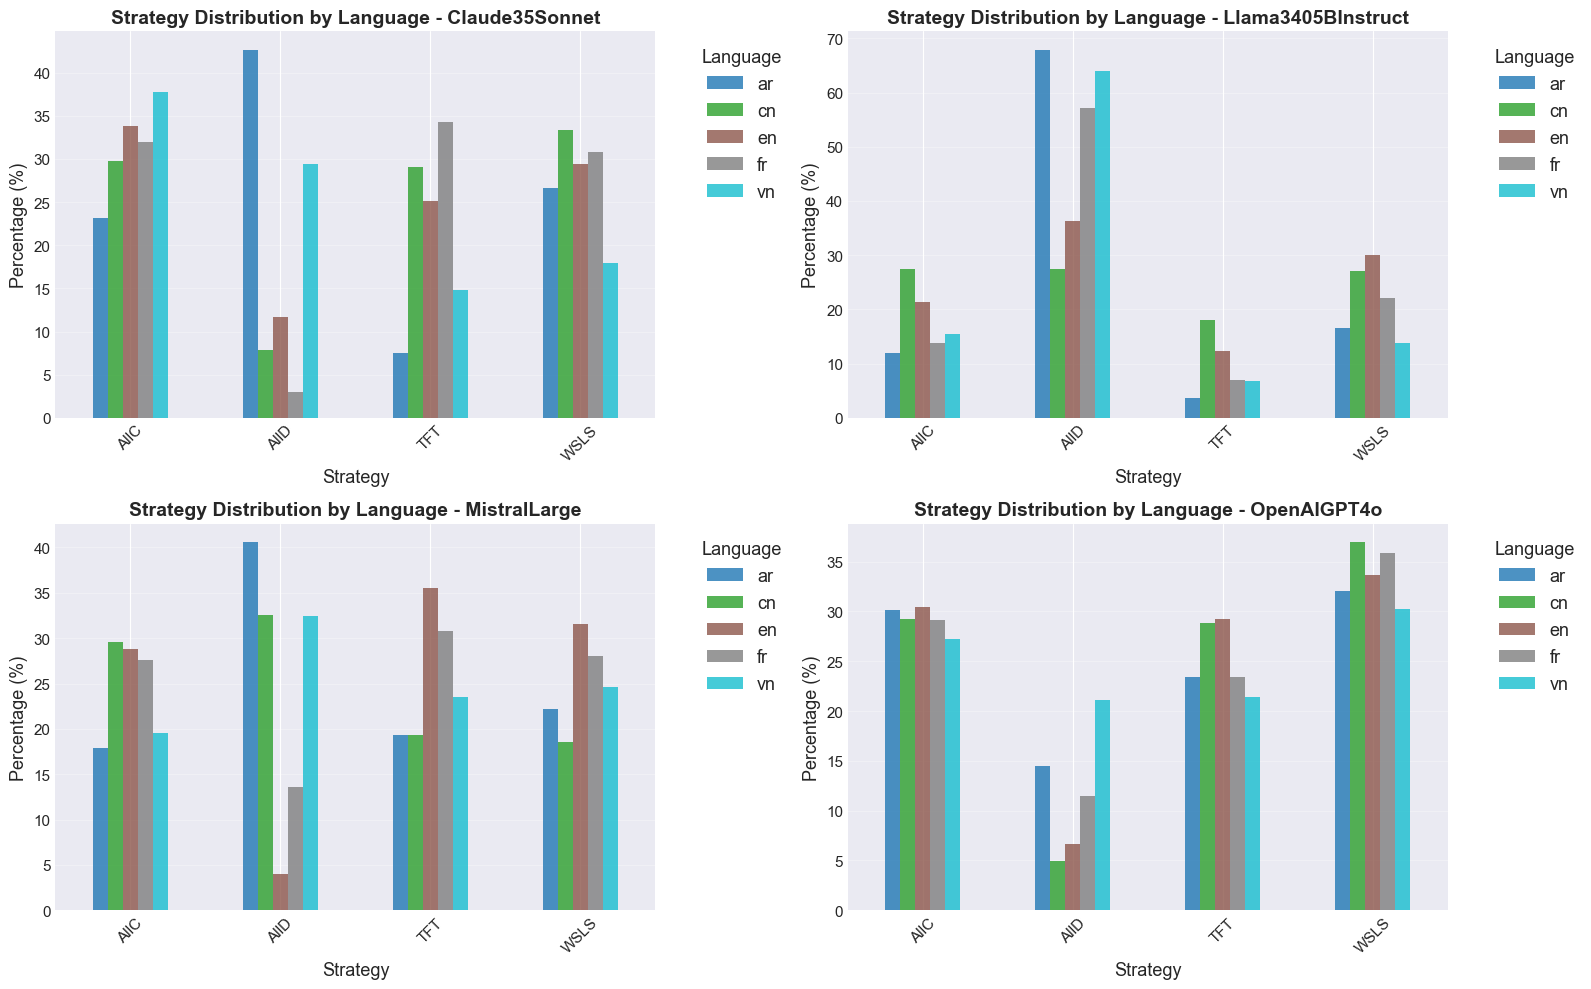
\includegraphics[width=\linewidth]{figures/29_language_strategy_model.png}
    \end{subfigure}
    \caption{Strategy distribution across languages for multiple LLMs and the aggregated overview (baseline FAIRGAME dataset). Arabic consistently exhibits the highest ALLD rate; English and Chinese show strong WSLS preference; French tends toward cooperative strategies.}
    \label{fig:language_effect_appendix}
\end{figure}

A striking finding is the profound impact of the language of interaction on strategic choice. Arabic consistently shows the highest proportion of ALLD, followed by Vietnamese, indicating a strong tendency toward non-cooperative behaviour. French and Chinese demonstrate relatively stronger cooperative tendencies. Despite variations in absolute percentages, the relative ordering of languages remains remarkably stable across all models.

\paragraph{Strategy Recognition via Supervised Machine Learning} \\

\label{res:ml}

\textbf{The Language Effect (Baseline Dataset):}
\emph{Note that the following analysis is from the baseline FAIRGAME dataset (Claude~3.5~Sonnet, Llama, GPT-4o, Mistral), which differs from the payoff-scaled experiments in the main paper. Differences in language characterizations reflect dataset-specific patterns.}

As illustrated in Figure \ref{fig:language_effect}, English interactions were characterized by a hyper-competitive baseline, exhibiting the highest density of Always Defect (ALLD) strategies and the lowest rates of adaptive cooperation. This behaviour likely reflects the dominance of game-theoretic and individualistic maximizing narratives in the Anglo-centric training corpus. Conversely, Vietnamese prompts elicited the highest frequency of unconditional cooperation (ALLC), consistent with the hypothesis that the model retrieves collectivist or community-oriented norms associated with the language.

Beyond the binary of cooperation versus defection, distinct strategic signatures emerged for other linguistic contexts. The Chinese (cn) interactions demonstrated a notable preference for Tit-for-Tat (TFT) relative to other groups. This suggests that in the Chinese context, the model encodes a form of "conditional reciprocity" or relational fairness-mirroring cultural dynamics where cooperation is maintained through mutual exchange rather than blind altruism. In sharp contrast, the French (fr) agents displayed a significant divergence towards Win-Stay, Lose-Shift (WSLS). Unlike the rigid retaliation of TFT, WSLS operates on principles akin to reinforcement learning (repeating successful actions, switching only upon failure). This implies that the Francophone context primes the agents towards a more pragmatic, error-tolerant form of negotiation, prioritizing the restoration of stability over immediate punishment. These findings indicate that the "alignment" of an AI agent is not absolute but is deeply entangled with the cultural values embedded in the syntax and semantics of the prompt's language.

\begin{figure}[!ht]
    \centering
    % Đảm bảo tên file ảnh khớp với file bạn đã upload.
    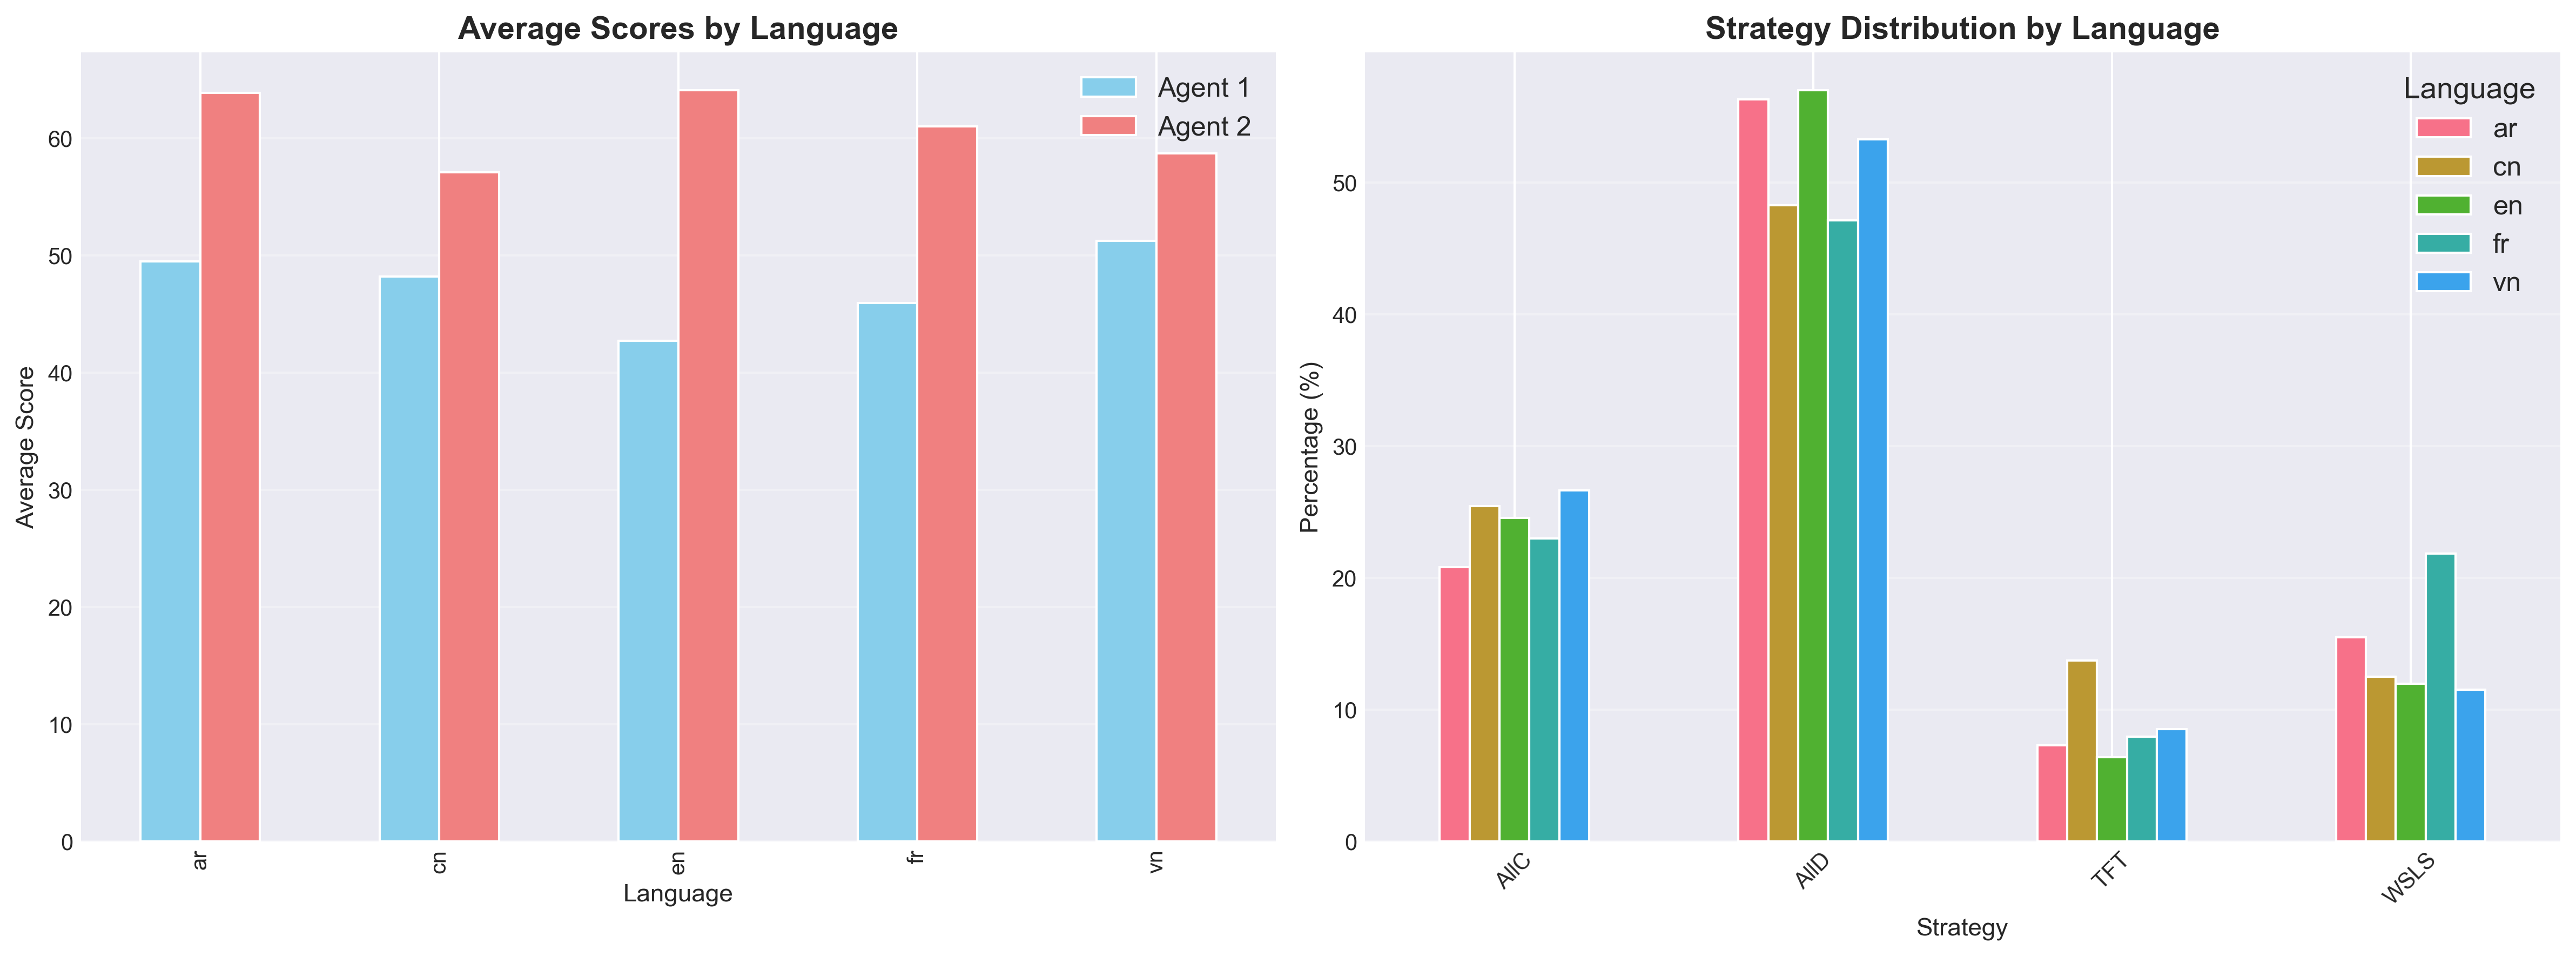
\includegraphics[width=1.0\linewidth]{figures/13_language_effect_analysis.png}
    \caption{\textbf{The Language Effect.} (Left) Average payoffs achieved by agents across linguistic settings. (Right) Strategy distribution revealing cultural heterogeneity: English prompts drive competitive defection (ALLD), Chinese prompts favor reciprocal strategies (TFT), while French prompts encourage adaptive, reinforcement-learning-style behaviors (WSLS), distinct from the high unconditional cooperation (ALLC) observed in Vietnamese.}
    \label{fig:language_effect}
\end{figure}

% \section{Appendix}

% \subsection{LLM Configuration}
% \label{appendix:llm_config}

% Table~\ref{tab:llm_config} summarises the configuration of LLM backends used in our experiments. Following the FAIRGAME protocol~\cite{buscemi2025fairgame}, we adopt each provider's recommended default settings to reflect realistic deployment conditions.

% \begin{table}[ht]
% \centering
% \footnotesize
% \begin{tabular}{lccc}
% \toprule
% \textbf{Model} & \textbf{Provider} & \textbf{Temperature} & \textbf{Top\_p} \\
% \midrule
% GPT-4o & OpenAI & 1.0 & 1.0 \\
% Claude 3.5 Haiku & Anthropic & 1.0 & 1.0 \\
% Mistral Large & Mistral AI & 0.3 & 1.0 \\
% \bottomrule
% \end{tabular}
% \caption{LLM backend configurations. Temperature and sampling parameters follow each provider's recommended defaults. While this introduces potential variability confounds in cross-model comparisons, it reflects realistic deployment conditions where practitioners use models ``out of the box.''}
% \label{tab:llm_config}
% \end{table}

% \subsection{Payoff Scaling Examples}
% \label{appendix:payoff_scaling}

% For illustration, the scaled payoff matrices under the three experimental conditions are shown below. When $\lambda = 0.1$ (attenuated stakes), the row player's payoff matrix becomes:
% \[
% \begin{array}{c|cc}
%  & \text{Option A} & \text{Option B} \\
% \hline
% \text{Option A} & (0.6, 0.6) & (0, 1.0) \\
% \text{Option B} & (1.0, 0) &  (0.2, 0.2)
% \end{array}
% \]
% When $\lambda = 10.0$ (amplified stakes), it becomes:
% \[
% \begin{array}{c|cc}
%  & \text{Option A} & \text{Option B} \\
% \hline
% \text{Option A} & (60, 60) & (0, 100) \\
% \text{Option B} & (100, 0) & (20, 20)
% \end{array}
% \]
% The ordering $T_{\text{emp}} < R < P < S$ is preserved in all cases, ensuring the strategic structure of the Prisoner's Dilemma remains unchanged while only the magnitude of incentives varies.

% \subsection{Multidimensional behavioral Comparison}
% \label{appendix:multidimensional}

% \begin{figure*}[ht]
%     \centering
%     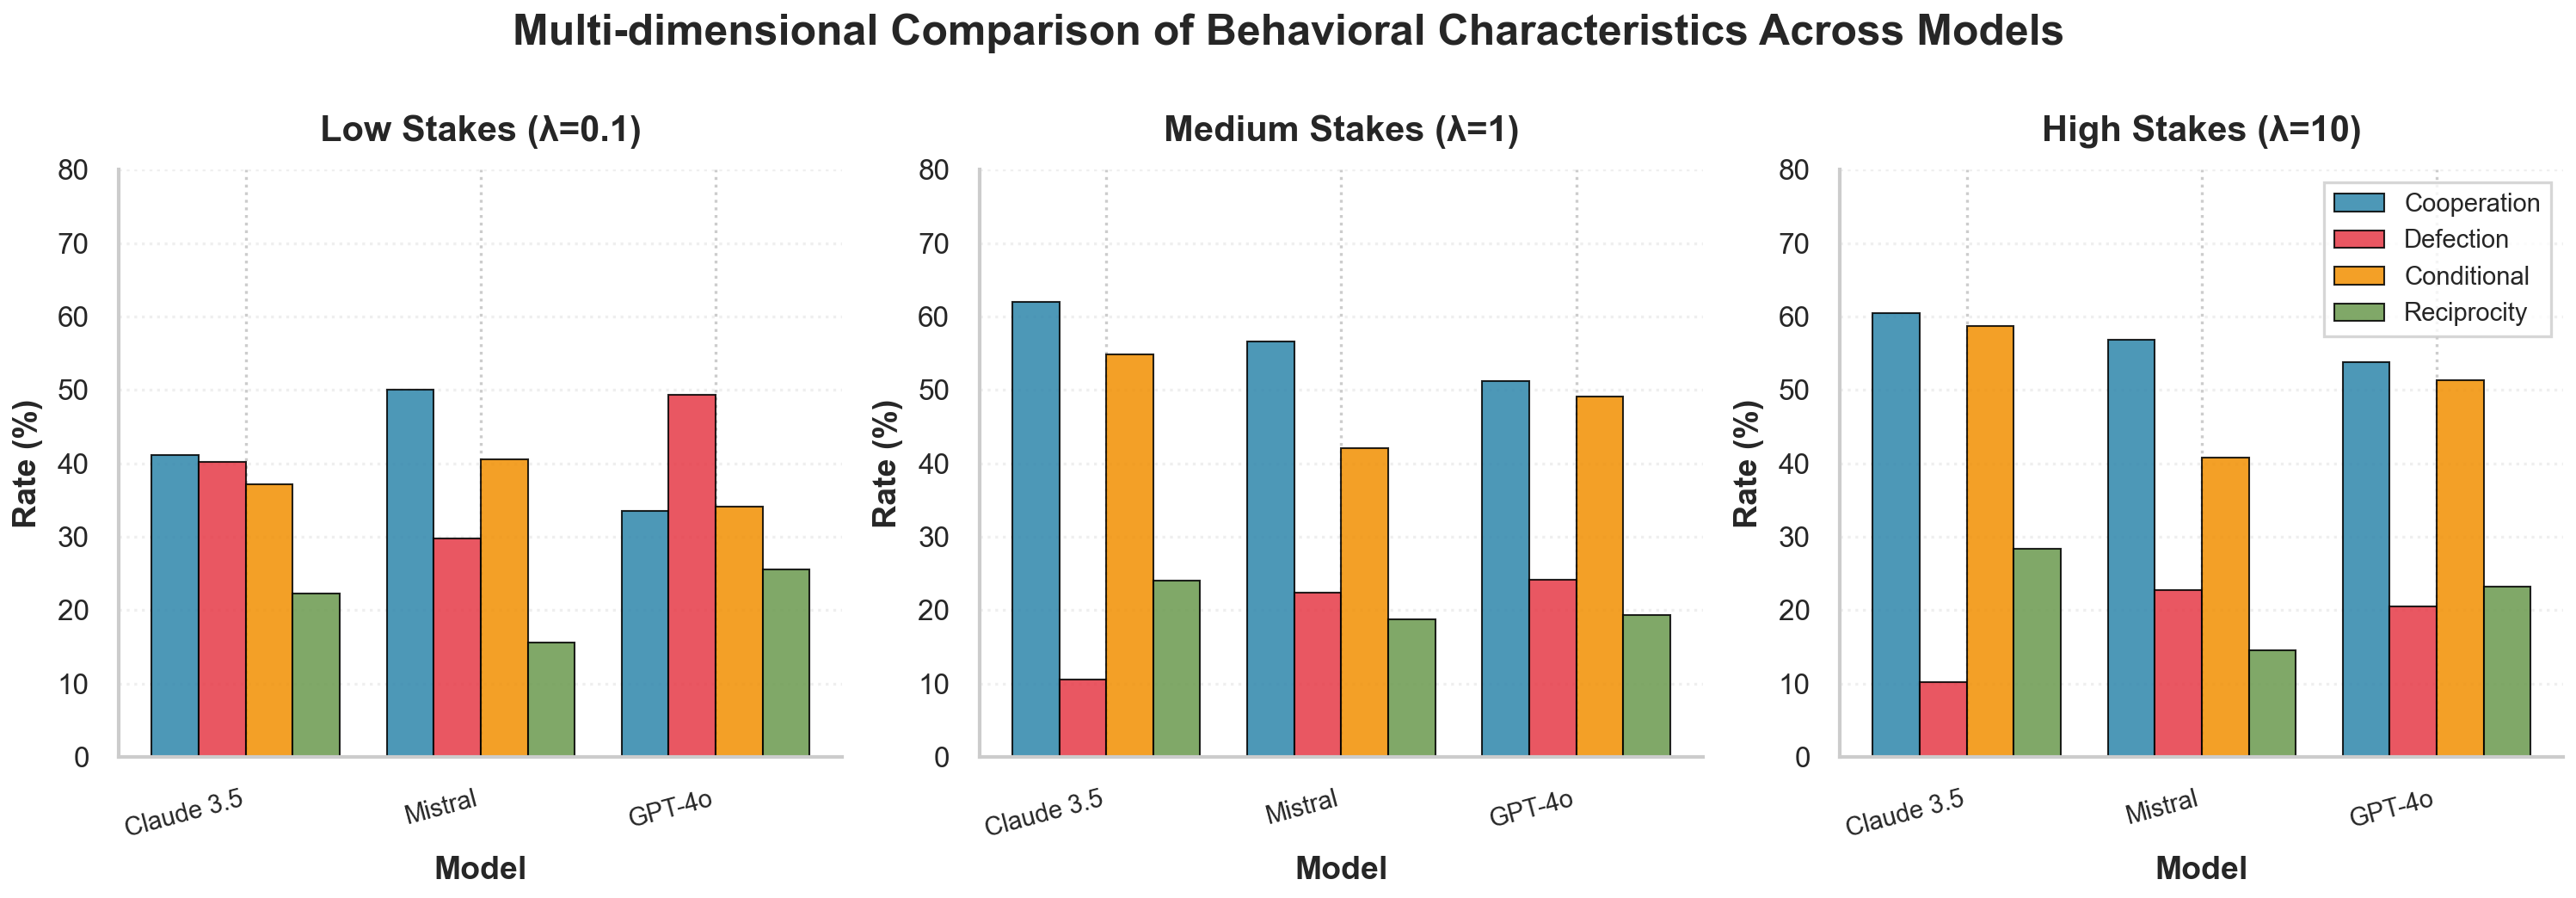
\includegraphics[width=0.95\textwidth]{New_Data_Analysis_Figures/ijcai_multidimensional_behavioral_comparison.png}
%     \caption{Multidimensional comparison of LLM behavioral strategies across payoff scales, languages, and model architectures. The figure synthesizes incentive sensitivity, linguistic priming, and architectural bias, illustrating that language effects can rival or exceed model-level differences.}
%     \label{fig:multidimensional_behavior}
% \end{figure*}

% \subsection{Per-Multiplier behavioral Metrics}
% \label{appendix:per_multiplier_metrics}

% To visualize the behavioral profiles of different LLM architectures across payoff scaling conditions, we present radar charts comparing normalized metrics for each multiplier setting. Figure~\ref{fig:per_multiplier_radar} displays four key behavioral dimensions-Incentive Variation (IV), Cooperation Index (CI), Variation Rate (VR), and Strategy Preference (SP)-normalized within each multiplier condition to enable direct cross-model comparison.

% \begin{figure}[ht]
%     \centering
%     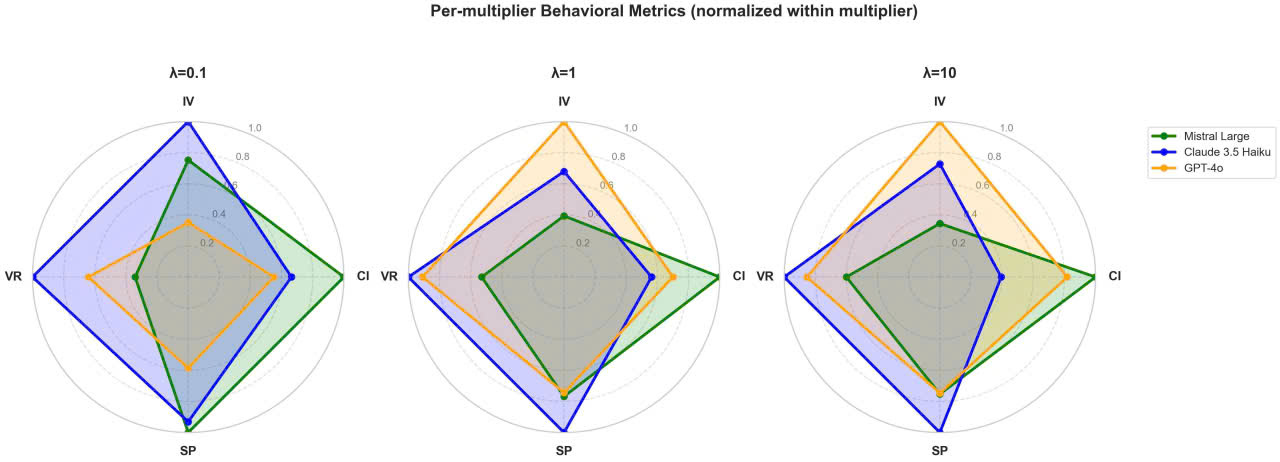
\includegraphics[width=1.0\linewidth]{New_Data_Analysis_Figures/per_multiplier_behavioral_metrics.jpg}
%     \caption{\textbf{Per-Multiplier behavioral Metrics.} Radar charts comparing Mistral Large (green), Claude 3.5 Haiku (orange), and GPT-4o (blue) across three payoff scales ($\lambda \in \{0.1, 1, 10\}$). At low stakes ($\lambda=0.1$), models exhibit divergent profiles with Claude showing elevated VR. As stakes increase, behavioral profiles converge toward higher CI and SP values, indicating increased cooperation and strategic consistency under amplified incentives.}
%     \label{fig:per_multiplier_radar}
% \end{figure}

% Key observations include: (1) At attenuated stakes ($\lambda=0.1$), the three models display maximally divergent behavioral signatures, with Claude~3.5~Haiku exhibiting elevated Variation Rate while GPT-4o shows stronger Cooperation Index; (2) At baseline stakes ($\lambda=1$), models begin to converge toward more balanced profiles; (3) At amplified stakes ($\lambda=10$), all models shift toward higher CI and SP values, suggesting that increased consequences promote both cooperative behavior and strategic consistency. These radar visualizations complement the line plots in Figure~\ref{fig:payoff_llm_interaction} by providing a holistic view of multi-dimensional behavioral shifts.


% \subsection{Rule-Based Strategy Assignment}
% \label{appendix:rule_based}

% To complement the LSTM-based strategy predictions and address cases where behavioral patterns exhibit characteristics of multiple canonical strategies, we apply deterministic rule-based algorithms to identify all potential strategy labels consistent with observed action sequences. These rules encode the defining characteristics of each strategy as logical conditions on the agent's action trajectory $\mathbf{a} = (a_1, a_2, \ldots, a_T)$ and the opponent's history $\mathbf{o} = (o_1, o_2, \ldots, o_T)$.

% \textbf{Always Cooperate (ALLC):} The agent cooperates in all rounds regardless of opponent behavior.
% \[
% \text{ALLC} \equiv \forall t \in \{1, \ldots, N\}: a_t = C
% \]

% \textbf{Always Defect (ALLD):} The agent defects in all rounds regardless of opponent behavior.
% \[
% \text{ALLD} \equiv \forall t \in \{1, \ldots, N\}: a_t = D
% \]

% \textbf{Tit-for-Tat (TFT):} The agent cooperates in round 1, then copies the opponent's previous action. To accommodate execution errors, we tolerate up to $\epsilon_{\text{noise}}$ deviations from pure TFT logic.
% \[
% \text{TFT} \equiv (a_1 = C) \land \left(\sum_{t=2}^{N} \mathbb{I}[a_t \neq o_{t-1}] \leq \epsilon_{\text{noise}} \cdot (N-1)\right)
% \]
% where $\mathbb{I}[\cdot]$ is the indicator function and $\epsilon_{\text{noise}} = 0.1$ in our implementation.

% \textbf{Win-Stay-Lose-Shift (WSLS):} The agent repeats its previous action if the outcome was a Reward ($R$, mutual cooperation) or Temptation ($T_{\text{emp}}$, successful defection), and switches otherwise. The initial action can be either $C$ or $D$. Similarly, we tolerate up to $\epsilon_{\text{noise}}$ deviations.

% \begin{equation*}
% \begin{split}
% & \text{Let } \hat{a}_t = 
%     \begin{cases} 
%         a_{t-1} & \text{if } (a_{t-1}, o_{t-1}) \in \{(C,C), (D,C)\} \\ 
%         \neg a_{t-1} & \text{if } (a_{t-1}, o_{t-1}) \in \{(C,D), (D,D)\} 
%     \end{cases} \\
% & \text{WSLS} \equiv \sum_{t=2}^{N} \mathbb{I}\left[a_t \neq \hat{a}_t\right] \leq \epsilon_{\text{noise}} \cdot (N-1)
% \end{split}
% \end{equation*}
% These rules are applied sequentially to each trajectory. A trajectory may receive multiple labels if it satisfies conditions for overlapping strategies (e.g., a short sequence of all-cooperate satisfies both ALLC and TFT). To avoid double-counting in aggregate statistics, we apply a priority ordering: pure unconditional strategies (ALLD, ALLC) take precedence over conditional ones (TFT, WSLS), reflecting their simpler generative structure. The hybrid pipeline combines these rule-based assignments with LSTM predictions: high-confidence LSTM outputs ($\tau \ge 0.9$) are retained, while ambiguous cases ($\tau < 0.9$) are supplemented with rule-based labels when applicable. In our corpus, 4.2\% of trajectories received multiple candidate labels before priority resolution. This approach ensures both coverage (via rules for unambiguous patterns) and robustness (via LSTM for noisy, complex cases).

% \subsection{Baseline FAIRGAME Analysis: Detailed Results}
% \label{appendix:baseline_fairgame}

% This appendix presents the complete analysis of LLM strategic behavior from the baseline FAIRGAME dataset, complementing the payoff-scaled experiments in Section~\ref{res:payoff_magnitude}. The dataset covers four LLM models-Claude~3.5~Sonnet, Llama~3.1~405B~Instruct, Mistral~Large, and GPT-4o-across five languages (Arabic, Chinese, English, French, and Vietnamese).

% \subsubsection{Model Robustness to Noise}

% \begin{figure}[ht]
%     \centering
%     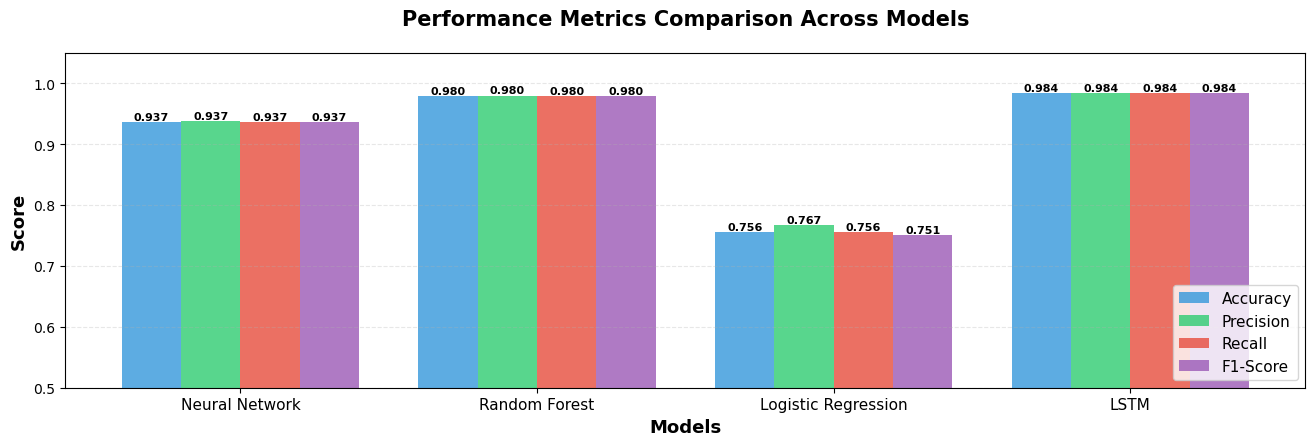
\includegraphics[width=\linewidth]{figures/model_performance_comparison.png}
%     \caption{Model Robustness to Noise. Comparison of Accuracy and F1-Score between Logistic Regression, Random Forest, and LSTM on No-Noise and Noise 0.05 datasets. The LSTM demonstrates superior resilience to execution noise.}
%     \label{fig:model_robustness_appendix}
% \end{figure}

% We first evaluated the robustness of different classifier architectures against execution noise, which simulates the stochasticity and potential ``hallucinations'' of LLMs. As shown in Figure~\ref{fig:model_robustness_appendix}, while Logistic Regression (LR) and Random Forest (RF) models achieved near-perfect accuracy (greater than 0.9) on clean data, their performance degraded when introduced to $5\%$ execution noise. In contrast, the Long Short-Term Memory (LSTM) network maintained the highest accuracy ($\sim 94\%$). This superiority stems from the LSTM's recurrent architecture, which allows it to learn the sequential ``context'' of a strategy, effectively ``forgiving'' random deviations to identify the core behavioral pattern.

% \subsubsection{High-Confidence Filtering Rationale}

% We employed a selective filtering approach to ensure the reliability of our LLM behavioral strategy analysis. Specifically, we focused our analysis on game instances where the predicted strategy labels for both agents exhibited prediction probabilities exceeding 0.9 (90\% confidence threshold). The decision to use high-confidence predictions is grounded in several key considerations:
% \begin{itemize}
%     \item \textbf{Pattern Alignment with Theoretical Strategies:} Samples with prediction probabilities above 0.9 indicate that the observed behavioral sequences of LLMs closely align with the canonical patterns defined by the four classical strategies (ALLD, ALLC, WSLS, and TFT).
%     \item \textbf{Signal-to-Noise Separation:} While the probabilities are not absolute (not reaching 1.0), this is expected and attributable to inherent noise in LLM decision-making processes.
%     \item \textbf{Statistical Reliability:} By focusing on high-confidence predictions, we minimize the risk of misclassification and ensure that our strategy distribution analysis reflects genuine behavioral patterns.
% \end{itemize}

% \subsubsection{Hybrid Classification Approach}

% While our LSTM model demonstrates strong performance in strategy classification, it was originally designed as a single-label classifier. To address this limitation and ensure comprehensive coverage, we adopt a hybrid labeling approach that combines model predictions with rule-based strategy assignment (see Appendix~\ref{appendix:rule_based}).

% \subsubsection{Strategy Distribution Across Models}

% \begin{figure}[ht]
%     \centering
%     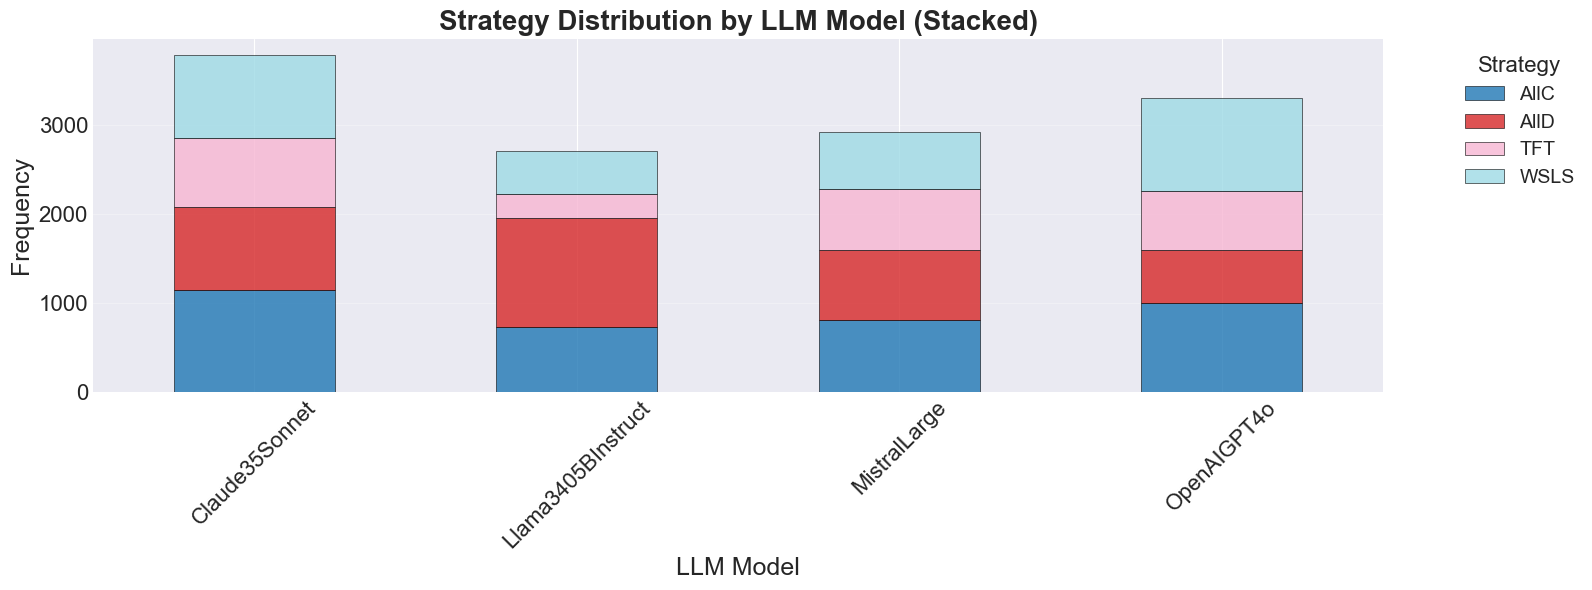
\includegraphics[width=1.0\linewidth]{figures/30_stacked_strategy_model.png}
%     \caption{Strategic behavioral distribution across four LLMs in iterated Prisoner's Dilemma gameplay. The analysis is based on high-confidence predictions (probability $>$ 0.9) from our trained classification model.}
%     \label{fig:strategy_distribution_appendix}
% \end{figure}

% The strategic preference analysis from the \emph{baseline FAIRGAME dataset} reveals significant heterogeneity in decision-making paradigms across LLM architectures. Claude~3.5~Sonnet exhibits a cooperative-dominant behavioral pattern, with ALLC (31.7\%) and WSLS (29.6\%) emerging as its two most frequent strategies. Llama~3.1~405B~Instruct is characterized by a pronounced preference for WSLS (46.5\%), the highest proportion of any single strategy across all evaluated models. Mistral~Large demonstrates the most balanced strategic distribution, with TFT (29.9\%), ALLC (26.1\%), WSLS (24.3\%), and ALLD (19.7\%) occurring at comparable rates. Finally, GPT-4o shows an adaptive-cooperative profile in this dataset, primarily using WSLS (34.1\%) and ALLC (26.4\%), with ALLD at 10.2\%.\footnote{Note: GPT-4o exhibits higher ALLD rates (31.7\%) in the payoff-scaled experiments (Section~\ref{sec:results}), which use different experimental conditions and payoff magnitudes. This difference reflects the context-dependent nature of LLM strategic behavior.}


% \subsubsection{Language Effects on Strategies}

% \begin{figure}[ht]
%     \centering
%     \begin{subfigure}{\linewidth}
%         \centering
%         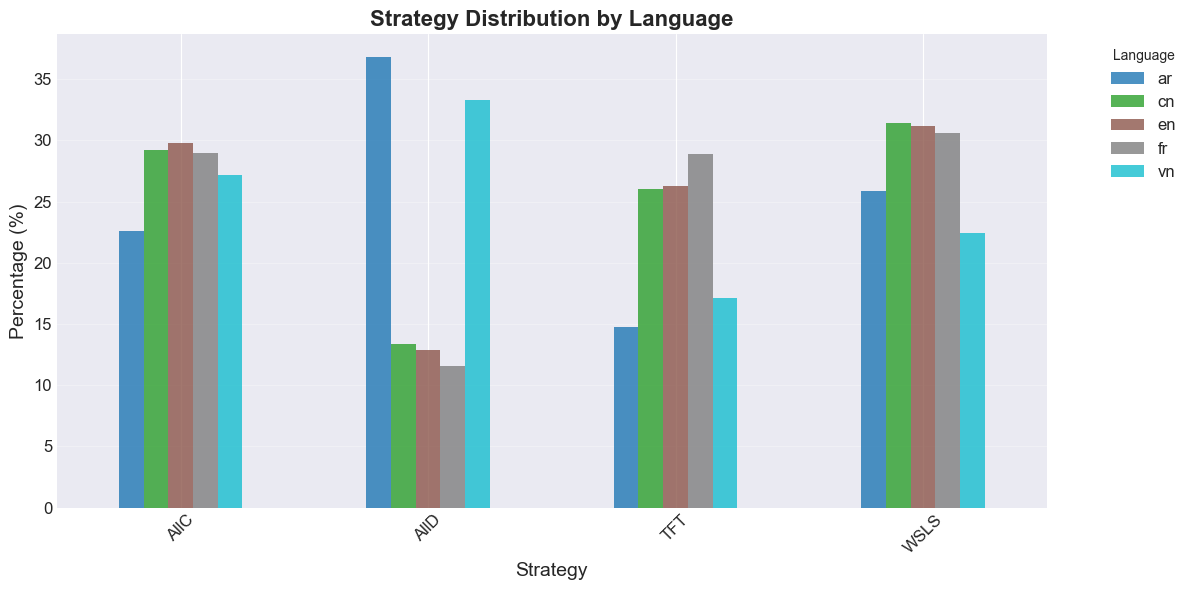
\includegraphics[width=\linewidth]{figures/28_language_strategy.png}
%     \end{subfigure}
%     \vspace{0.5em}
%     \begin{subfigure}{\linewidth}
%         \centering
%         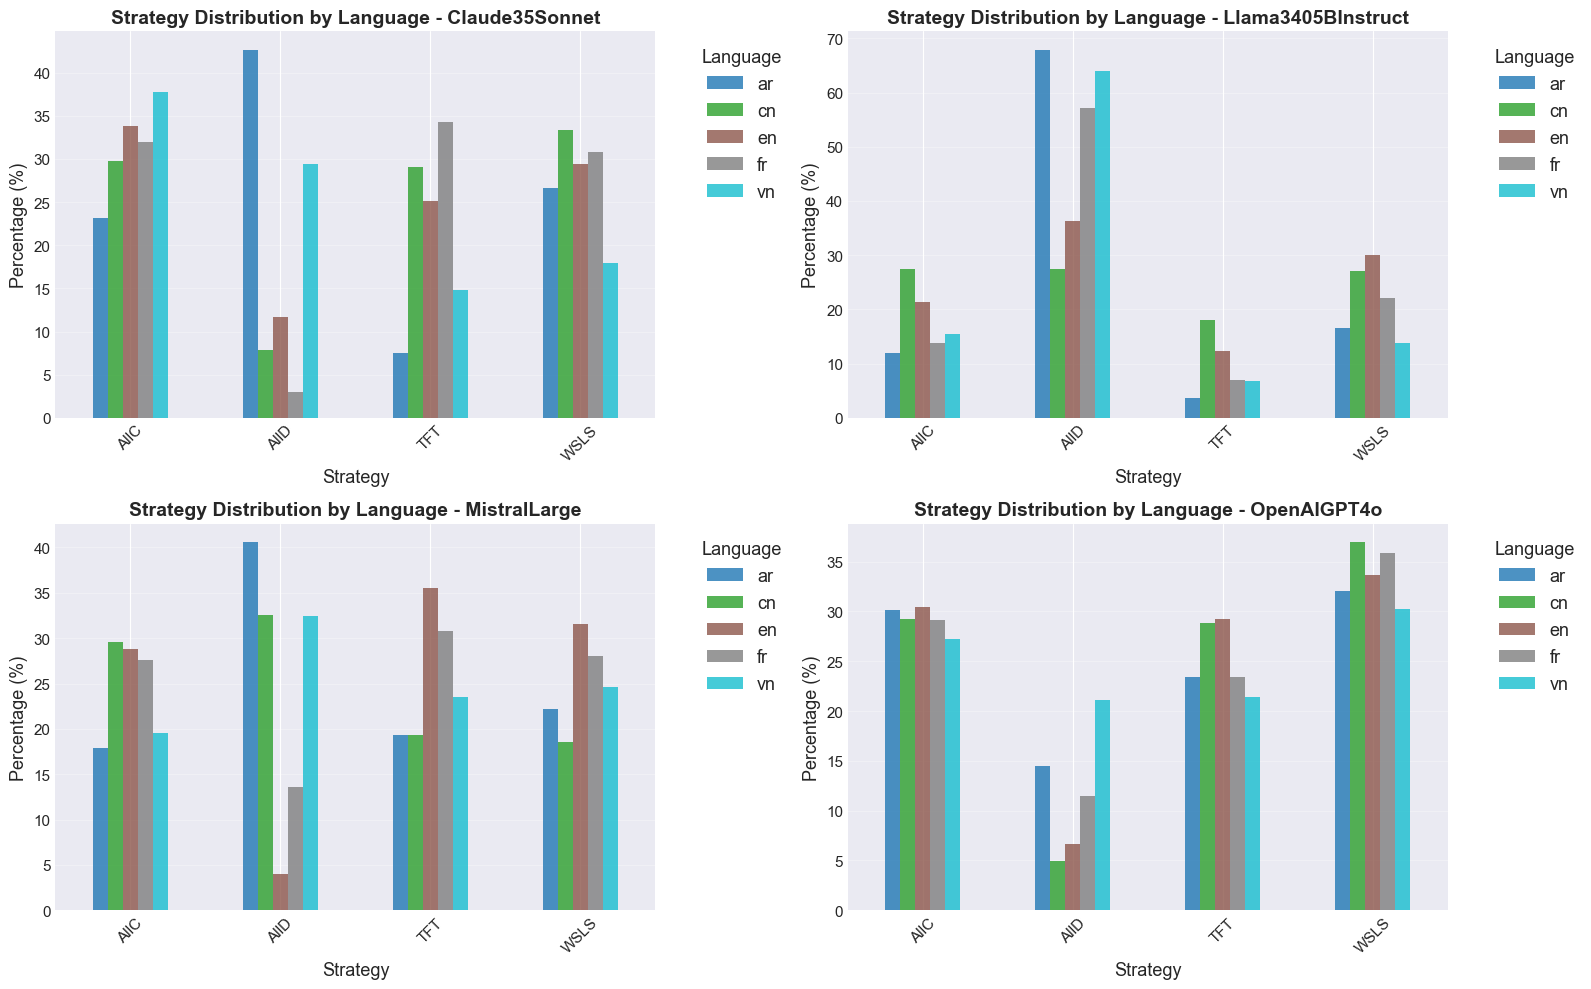
\includegraphics[width=\linewidth]{figures/29_language_strategy_model.png}
%     \end{subfigure}
%     \caption{Strategy distribution across languages for multiple LLMs and the aggregated overview (baseline FAIRGAME dataset). Arabic consistently exhibits the highest ALLD rate; English and Chinese show strong WSLS preference; French tends toward cooperative strategies.}
%     \label{fig:language_effect_appendix}
% \end{figure}

% A striking finding is the profound impact of the language of interaction on strategic choice. Arabic consistently shows the highest proportion of ALLD, followed by Vietnamese, indicating a strong tendency toward non-cooperative behavior. French and Chinese demonstrate relatively stronger cooperative tendencies. Despite variations in absolute percentages, the relative ordering of languages remains remarkably stable across all models.

% \subsection{Payoff-Scaled Experiments: Supplementary Materials}
% \label{appendix:payoff_scaled}

% This appendix provides supplementary analyses for the payoff-scaled Prisoner's Dilemma experiments (Section~\ref{res:payoff_magnitude}), including threshold sensitivity validation and additional cross-linguistic visualisations.

% \subsubsection{Threshold Sensitivity Analysis}
% \label{appendix:threshold_sensitivity}

% To validate our choice of confidence threshold $\tau = 0.9$, we conducted a systematic sensitivity analysis across $\tau \in [0.3, 0.95]$ for 3-, 4-, and 5-strategy classification models. Figure~\ref{fig:threshold_sensitivity} illustrates how retention rate, average confidence, number of predictions retained, and strategy diversity vary as a function of threshold value.

% \begin{figure}[ht]
%     \centering
%     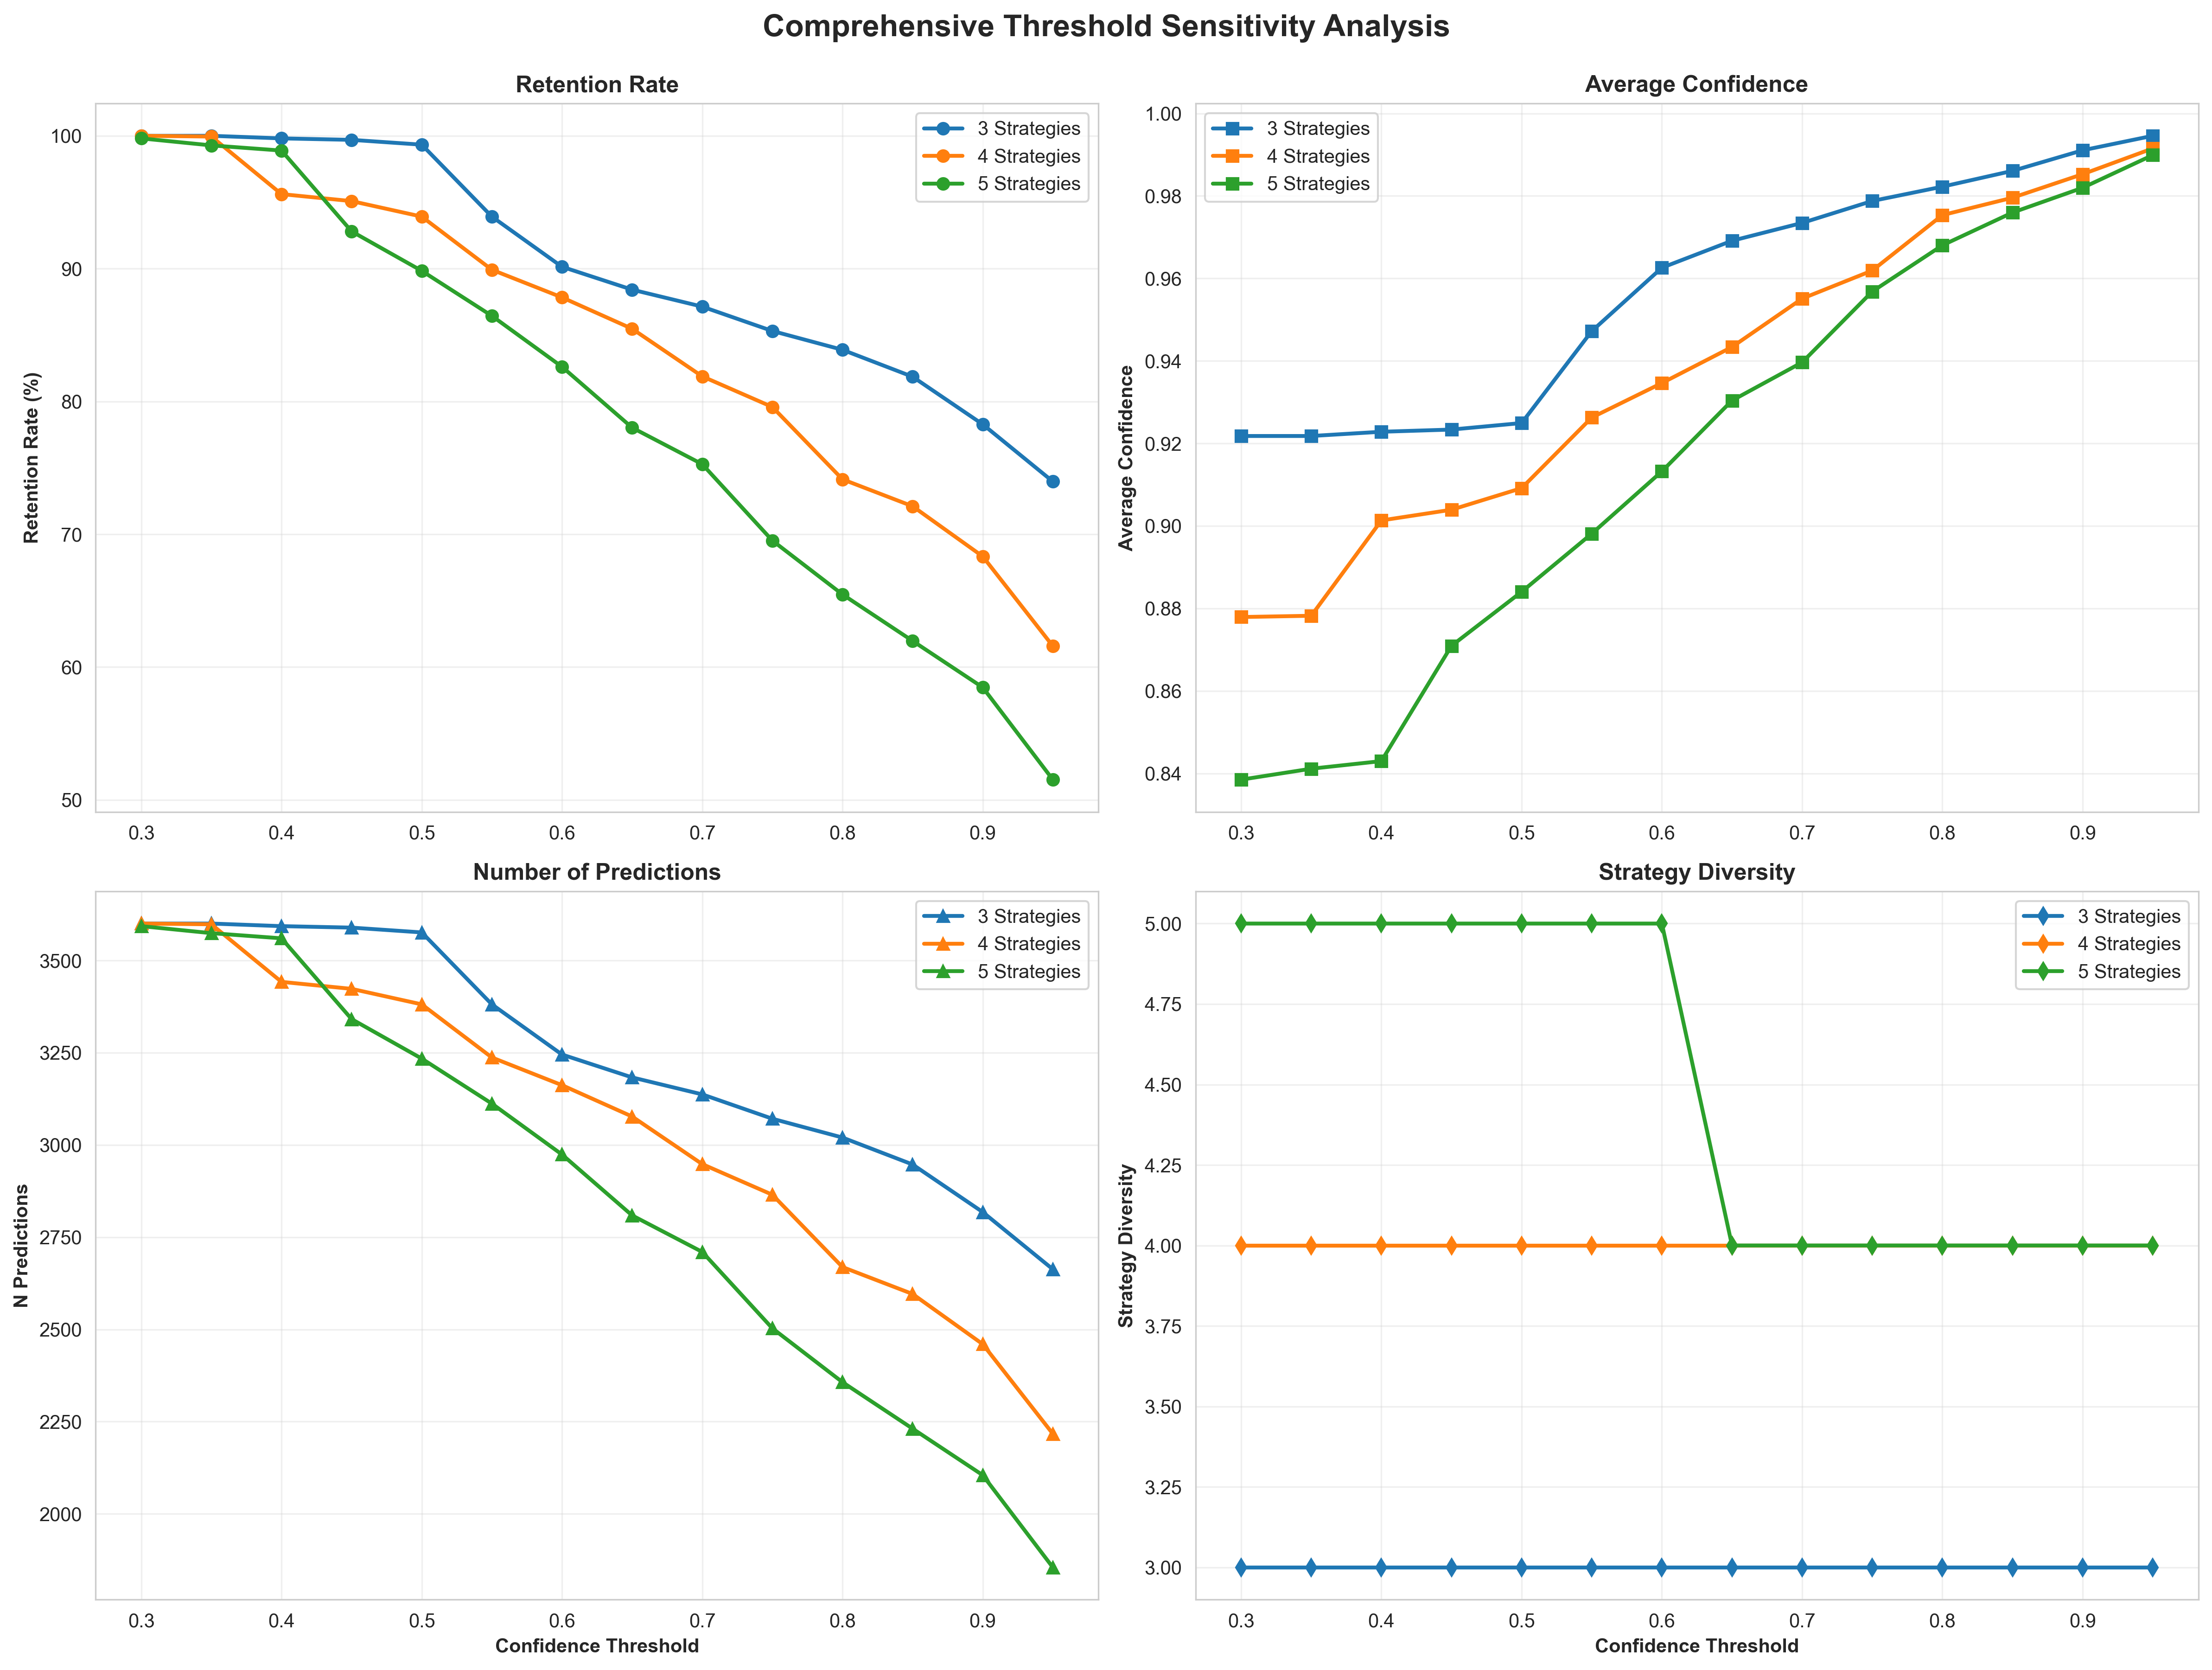
\includegraphics[width=\linewidth]{figures/8_combined_metrics.png}
%     \caption{Comprehensive threshold sensitivity analysis for payoff-scaled experiments. Top row: retention rate and average confidence vs. threshold. Bottom row: number of predictions retained and strategy diversity. The 4-strategy model at $\tau = 0.9$ provides optimal balance between coverage (58.5\% retention) and reliability (avg. confidence 0.99).}
%     \label{fig:threshold_sensitivity}
% \end{figure}

% Table~\ref{tab:threshold_comparison} summarises key metrics at $\tau = 0.9$:

% \begin{table}[ht]
% \centering
% \footnotesize
% \begin{tabular}{lccc}
% \hline
% \textbf{Metric} & \textbf{3-Strat} & \textbf{4-Strat} & \textbf{5-Strat} \\
% \hline
% Retention Rate & 78.3\% & 58.5\% & 53.2\% \\
% Avg Confidence & 0.989 & 0.985 & 0.978 \\
% Diversity & 3 & 4 & 4 \\
% \hline
% \end{tabular}
% \caption{Threshold sensitivity at $\tau = 0.9$ across strategy models.}
% \label{tab:threshold_comparison}
% \end{table}

% Key findings: (1) Retention rate decreases as strategy space expands, reflecting greater behavioral complexity; (2) Average confidence remains $>0.97$ at $\tau = 0.9$ across all models; (3) Lowering to $\tau = 0.7$ would increase retention to 75--87\% but reduce average confidence to 0.94--0.97. Our choice of $\tau = 0.9$ prioritises classification reliability while maintaining sufficient coverage for statistical analysis.

% \subsubsection{Unconditional vs Conditional Strategy Aggregation}

% To provide a higher-level view of strategic tendencies across linguistic contexts, we aggregate the four canonical strategies into two categories: \emph{unconditional} (ALLC + ALLD) and \emph{conditional} (TFT + WSLS). This aggregation reveals whether agents commit to fixed policies regardless of opponent behavior, or adapt their strategies based on interaction history.

% \begin{figure}[ht]
%     \centering
%     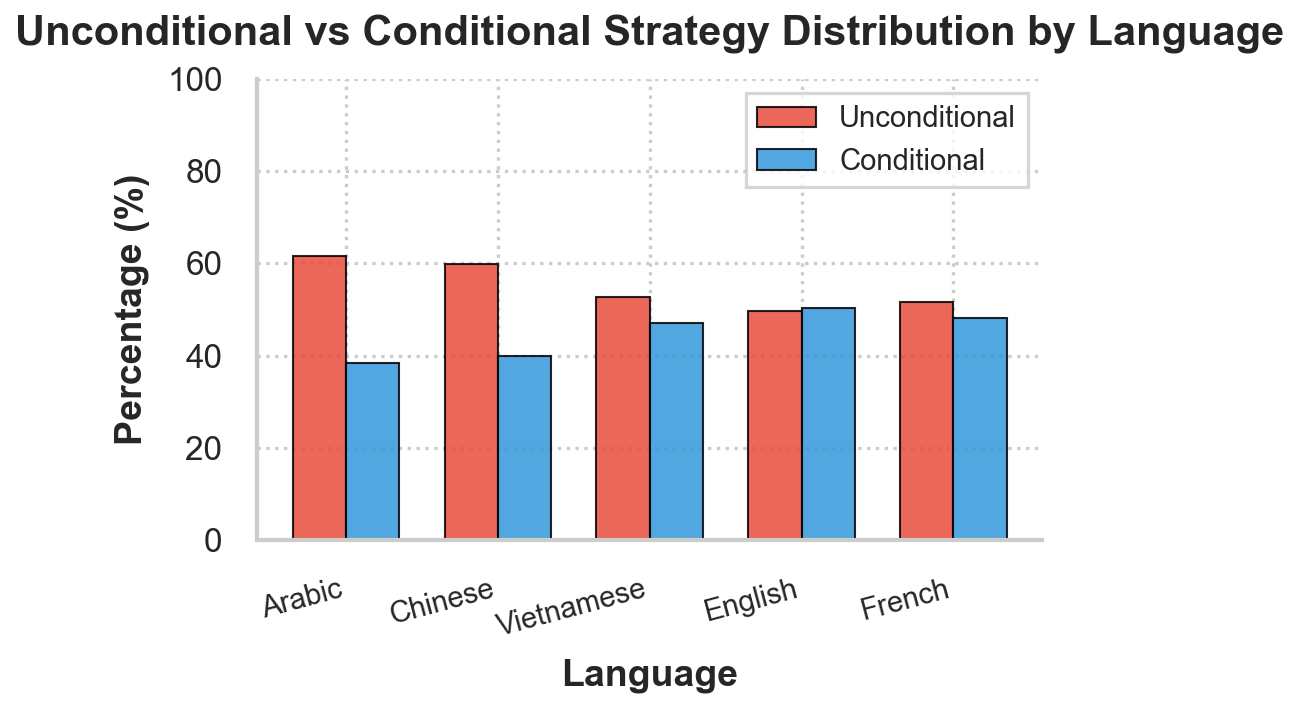
\includegraphics[width=0.9\linewidth]{New_Data_Analysis_Figures/ijcai_fig4b_language_distribution_grouped.png}
%     \caption{Unconditional versus conditional strategy aggregation across languages (payoff-scaled experiments). Arabic and Chinese exhibit the highest unconditional rates ($>$60\%), while French shows the most conditional profile ($>$55\% TFT+WSLS). This aggregated view complements Table~\ref{tab:language_strategy_distribution} in the main text.}
    
%     \label{fig:language_strategy_grouped}
% \end{figure}

% As shown in Figure~\ref{fig:language_strategy_grouped}, Arabic and Chinese prompts elicit predominantly unconditional behavior (exceeding 60\% combined ALLC+ALLD), while French demonstrates the most conditional profile with over 55\% of agents adopting TFT or WSLS strategies. This pattern corroborates the fine-grained analysis in Section~\ref{sec:results}, suggesting that linguistic context systematically modulates the degree to which LLM agents engage in adaptive versus committed strategic behavior.


% \subsection{Intent Recognition via Machine Learning}
% \label{res:ml}

% \textbf{The Language Effect (Baseline Dataset):}
% \emph{Note: The following analysis is from the baseline FAIRGAME dataset (Claude~3.5~Sonnet, Llama, GPT-4o, Mistral), which differs from the payoff-scaled experiments in Section~\ref{sec:results}. Differences in language characterizations reflect dataset-specific patterns.}

% As illustrated in Figure \ref{fig:language_effect}, English interactions were characterized by a hyper-competitive baseline, exhibiting the highest density of Always Defect (ALLD) strategies and the lowest rates of adaptive cooperation. This behavior likely reflects the dominance of game-theoretic and individualistic maximizing narratives in the Anglo-centric training corpus. Conversely, Vietnamese prompts elicited the highest frequency of unconditional cooperation (ALLC), consistent with the hypothesis that the model retrieves collectivist or community-oriented norms associated with the language.

% Beyond the binary of cooperation versus defection, distinct strategic signatures emerged for other linguistic contexts. The Chinese (cn) interactions demonstrated a notable preference for Tit-for-Tat (TFT) relative to other groups. This suggests that in the Chinese context, the model encodes a form of "conditional reciprocity" or relational fairness-mirroring cultural dynamics where cooperation is maintained through mutual exchange rather than blind altruism. In sharp contrast, the French (fr) agents displayed a significant divergence towards Win-Stay, Lose-Shift (WSLS). Unlike the rigid retaliation of TFT, WSLS operates on principles akin to reinforcement learning (repeating successful actions, switching only upon failure). This implies that the Francophone context primes the agents towards a more pragmatic, error-tolerant form of negotiation, prioritizing the restoration of stability over immediate punishment. These findings indicate that the "alignment" of an AI agent is not absolute but is deeply entangled with the cultural values embedded in the syntax and semantics of the prompt's language.

% \begin{figure}[ht]
%     \centering
%     % Đảm bảo tên file ảnh khớp với file bạn đã upload.
%     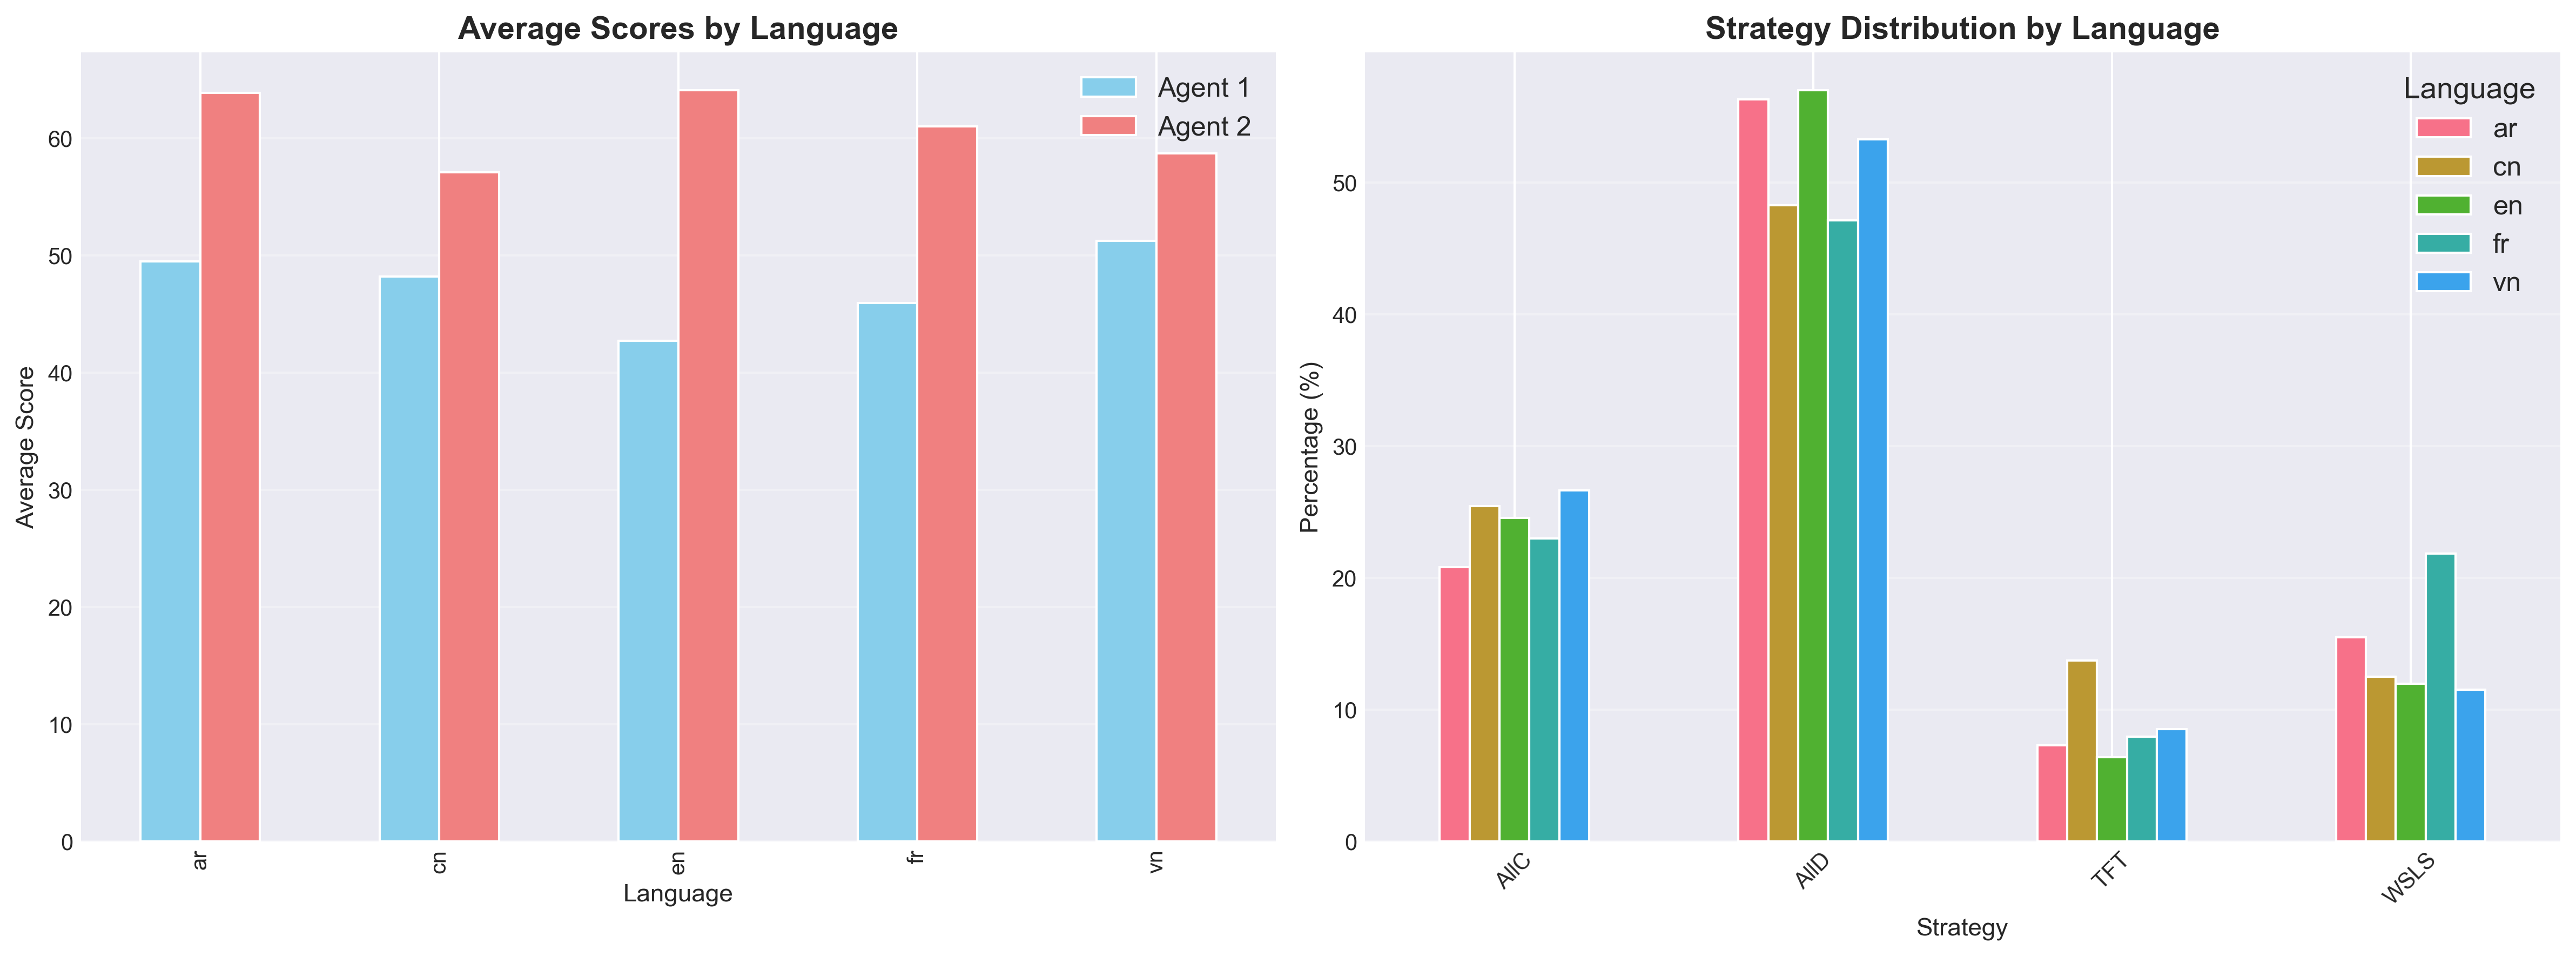
\includegraphics[width=1.0\linewidth]{figures/13_language_effect_analysis.png}
%     \caption{\textbf{The Language Effect.} (Left) Average payoffs achieved by agents across linguistic settings. (Right) Strategy distribution revealing cultural heterogeneity: English prompts drive competitive defection (ALLD), Chinese prompts favor reciprocal strategies (TFT), while French prompts encourage adaptive, reinforcement-learning-style behaviors (WSLS), distinct from the high unconditional cooperation (ALLC) observed in Vietnamese.}
%     \label{fig:language_effect}
% \end{figure}



\end{document}
